% Options for packages loaded elsewhere
\PassOptionsToPackage{unicode}{hyperref}
\PassOptionsToPackage{hyphens}{url}
%
\documentclass[
]{article}
\usepackage{amsmath,amssymb}
\usepackage{iftex}
\ifPDFTeX
  \usepackage[T1]{fontenc}
  \usepackage[utf8]{inputenc}
  \usepackage{textcomp} % provide euro and other symbols
\else % if luatex or xetex
  \usepackage{unicode-math} % this also loads fontspec
  \defaultfontfeatures{Scale=MatchLowercase}
  \defaultfontfeatures[\rmfamily]{Ligatures=TeX,Scale=1}
\fi
\usepackage{lmodern}
\ifPDFTeX\else
  % xetex/luatex font selection
\fi
% Use upquote if available, for straight quotes in verbatim environments
\IfFileExists{upquote.sty}{\usepackage{upquote}}{}
\IfFileExists{microtype.sty}{% use microtype if available
  \usepackage[]{microtype}
  \UseMicrotypeSet[protrusion]{basicmath} % disable protrusion for tt fonts
}{}
\makeatletter
\@ifundefined{KOMAClassName}{% if non-KOMA class
  \IfFileExists{parskip.sty}{%
    \usepackage{parskip}
  }{% else
    \setlength{\parindent}{0pt}
    \setlength{\parskip}{6pt plus 2pt minus 1pt}}
}{% if KOMA class
  \KOMAoptions{parskip=half}}
\makeatother
\usepackage{xcolor}
\usepackage[margin=1in]{geometry}
\usepackage{color}
\usepackage{fancyvrb}
\newcommand{\VerbBar}{|}
\newcommand{\VERB}{\Verb[commandchars=\\\{\}]}
\DefineVerbatimEnvironment{Highlighting}{Verbatim}{commandchars=\\\{\}}
% Add ',fontsize=\small' for more characters per line
\usepackage{framed}
\definecolor{shadecolor}{RGB}{248,248,248}
\newenvironment{Shaded}{\begin{snugshade}}{\end{snugshade}}
\newcommand{\AlertTok}[1]{\textcolor[rgb]{0.94,0.16,0.16}{#1}}
\newcommand{\AnnotationTok}[1]{\textcolor[rgb]{0.56,0.35,0.01}{\textbf{\textit{#1}}}}
\newcommand{\AttributeTok}[1]{\textcolor[rgb]{0.13,0.29,0.53}{#1}}
\newcommand{\BaseNTok}[1]{\textcolor[rgb]{0.00,0.00,0.81}{#1}}
\newcommand{\BuiltInTok}[1]{#1}
\newcommand{\CharTok}[1]{\textcolor[rgb]{0.31,0.60,0.02}{#1}}
\newcommand{\CommentTok}[1]{\textcolor[rgb]{0.56,0.35,0.01}{\textit{#1}}}
\newcommand{\CommentVarTok}[1]{\textcolor[rgb]{0.56,0.35,0.01}{\textbf{\textit{#1}}}}
\newcommand{\ConstantTok}[1]{\textcolor[rgb]{0.56,0.35,0.01}{#1}}
\newcommand{\ControlFlowTok}[1]{\textcolor[rgb]{0.13,0.29,0.53}{\textbf{#1}}}
\newcommand{\DataTypeTok}[1]{\textcolor[rgb]{0.13,0.29,0.53}{#1}}
\newcommand{\DecValTok}[1]{\textcolor[rgb]{0.00,0.00,0.81}{#1}}
\newcommand{\DocumentationTok}[1]{\textcolor[rgb]{0.56,0.35,0.01}{\textbf{\textit{#1}}}}
\newcommand{\ErrorTok}[1]{\textcolor[rgb]{0.64,0.00,0.00}{\textbf{#1}}}
\newcommand{\ExtensionTok}[1]{#1}
\newcommand{\FloatTok}[1]{\textcolor[rgb]{0.00,0.00,0.81}{#1}}
\newcommand{\FunctionTok}[1]{\textcolor[rgb]{0.13,0.29,0.53}{\textbf{#1}}}
\newcommand{\ImportTok}[1]{#1}
\newcommand{\InformationTok}[1]{\textcolor[rgb]{0.56,0.35,0.01}{\textbf{\textit{#1}}}}
\newcommand{\KeywordTok}[1]{\textcolor[rgb]{0.13,0.29,0.53}{\textbf{#1}}}
\newcommand{\NormalTok}[1]{#1}
\newcommand{\OperatorTok}[1]{\textcolor[rgb]{0.81,0.36,0.00}{\textbf{#1}}}
\newcommand{\OtherTok}[1]{\textcolor[rgb]{0.56,0.35,0.01}{#1}}
\newcommand{\PreprocessorTok}[1]{\textcolor[rgb]{0.56,0.35,0.01}{\textit{#1}}}
\newcommand{\RegionMarkerTok}[1]{#1}
\newcommand{\SpecialCharTok}[1]{\textcolor[rgb]{0.81,0.36,0.00}{\textbf{#1}}}
\newcommand{\SpecialStringTok}[1]{\textcolor[rgb]{0.31,0.60,0.02}{#1}}
\newcommand{\StringTok}[1]{\textcolor[rgb]{0.31,0.60,0.02}{#1}}
\newcommand{\VariableTok}[1]{\textcolor[rgb]{0.00,0.00,0.00}{#1}}
\newcommand{\VerbatimStringTok}[1]{\textcolor[rgb]{0.31,0.60,0.02}{#1}}
\newcommand{\WarningTok}[1]{\textcolor[rgb]{0.56,0.35,0.01}{\textbf{\textit{#1}}}}
\usepackage{graphicx}
\makeatletter
\newsavebox\pandoc@box
\newcommand*\pandocbounded[1]{% scales image to fit in text height/width
  \sbox\pandoc@box{#1}%
  \Gscale@div\@tempa{\textheight}{\dimexpr\ht\pandoc@box+\dp\pandoc@box\relax}%
  \Gscale@div\@tempb{\linewidth}{\wd\pandoc@box}%
  \ifdim\@tempb\p@<\@tempa\p@\let\@tempa\@tempb\fi% select the smaller of both
  \ifdim\@tempa\p@<\p@\scalebox{\@tempa}{\usebox\pandoc@box}%
  \else\usebox{\pandoc@box}%
  \fi%
}
% Set default figure placement to htbp
\def\fps@figure{htbp}
\makeatother
\setlength{\emergencystretch}{3em} % prevent overfull lines
\providecommand{\tightlist}{%
  \setlength{\itemsep}{0pt}\setlength{\parskip}{0pt}}
\setcounter{secnumdepth}{-\maxdimen} % remove section numbering
\usepackage{booktabs}
\usepackage{bookmark}
\IfFileExists{xurl.sty}{\usepackage{xurl}}{} % add URL line breaks if available
\urlstyle{same}
\hypersetup{
  pdftitle={Simulations of Trust Game},
  pdfauthor={Your Name},
  hidelinks,
  pdfcreator={LaTeX via pandoc}}

\title{Simulations of Trust Game}
\author{Your Name}
\date{2025-07-07}

\begin{document}
\maketitle

\section{Simulations of Trust Game}\label{simulations-of-trust-game}

In Berg's experiment, there does not seem to be a significant difference
in the amount sent by participants in the treatment group (those with
social history) compared to those without. Let \(Y_{1}\) and \(Y_{2}\)
be two random variables associated to the control/baseline and the
treatment group respectively. and \(\mathcal{Z} \subset  \mathcal{R}\)
and \(Y_{1}, Y_{2} \in \mathcal{R}\). Furthermore, let \(P_{Y_{1}}\) and
\(P_{Y_{2}}\) be the probability distributions of \(Y_{1}\) and
\(Y_{2}\) respectively.

There is not statistical evidence to reject any of the following null
hypothesis:

\begin{itemize}
\tightlist
\item
  \(H_0\): The distribution of amounts sent is the same for both groups,
  i.e., \(H_{0}: Y_1 \overset{d}{=} Y_{2}\).
\item
  \(H_0\): The mean amount sent is the same for both groups, i.e.,
  \(\mathbb{E}[Y_{1}] = \mathbb{E}[Y_{2}]\).
\item
  \(H_0\): The probability that a randomly chosen individual from the
  treatment group sends more than one from the control group is 0.5,
  i.e., \(P(Y_{2} > Y_{1}) = P(Y_{1} > Y_{2}) = 0.5\).
\end{itemize}

\begin{Shaded}
\begin{Highlighting}[]
\CommentTok{\# No output is produced by loading the ggplot2 library, so nothing will be printed.}
\FunctionTok{library}\NormalTok{(exactRankTests)}
\FunctionTok{library}\NormalTok{(ggplot2)}
\FunctionTok{library}\NormalTok{(ggthemes)   }\CommentTok{\# Optional for extra themes}
\FunctionTok{library}\NormalTok{(scales)}
\FunctionTok{library}\NormalTok{(progress) }
\FunctionTok{library}\NormalTok{(knitr)}
\FunctionTok{library}\NormalTok{(readxl)}
\FunctionTok{library}\NormalTok{(dplyr)}

\FunctionTok{source}\NormalTok{(}\StringTok{"si.test.R"}\NormalTok{)}

\NormalTok{berg\_1995 }\OtherTok{\textless{}{-}} \FunctionTok{data.frame}\NormalTok{(}
  \AttributeTok{treatment =} \FunctionTok{c}\NormalTok{(}
    \FunctionTok{rep}\NormalTok{(}\DecValTok{0}\NormalTok{, }\DecValTok{32}\NormalTok{),  }\CommentTok{\# No History}
    \FunctionTok{rep}\NormalTok{(}\DecValTok{1}\NormalTok{, }\DecValTok{28}\NormalTok{)   }\CommentTok{\# Social History}
\NormalTok{  ),}
  \AttributeTok{sent =} \FunctionTok{c}\NormalTok{(}
    \DecValTok{7}\NormalTok{, }\DecValTok{3}\NormalTok{, }\DecValTok{7}\NormalTok{, }\DecValTok{5}\NormalTok{, }\DecValTok{3}\NormalTok{, }\DecValTok{2}\NormalTok{, }\DecValTok{6}\NormalTok{, }\DecValTok{4}\NormalTok{, }\DecValTok{10}\NormalTok{, }\DecValTok{5}\NormalTok{, }\DecValTok{5}\NormalTok{, }\DecValTok{10}\NormalTok{, }\DecValTok{5}\NormalTok{, }\DecValTok{8}\NormalTok{, }\DecValTok{5}\NormalTok{, }\DecValTok{0}\NormalTok{, }\DecValTok{7}\NormalTok{, }\DecValTok{1}\NormalTok{, }\DecValTok{3}\NormalTok{, }\DecValTok{2}\NormalTok{, }\DecValTok{6}\NormalTok{, }\DecValTok{10}\NormalTok{, }\DecValTok{3}\NormalTok{, }\DecValTok{6}\NormalTok{, }\DecValTok{6}\NormalTok{, }\DecValTok{10}\NormalTok{, }\DecValTok{10}\NormalTok{, }\DecValTok{6}\NormalTok{, }\DecValTok{4}\NormalTok{, }\DecValTok{0}\NormalTok{, }\DecValTok{5}\NormalTok{, }\DecValTok{1}\NormalTok{,}
    \DecValTok{5}\NormalTok{, }\DecValTok{10}\NormalTok{, }\DecValTok{2}\NormalTok{, }\DecValTok{5}\NormalTok{, }\DecValTok{0}\NormalTok{, }\DecValTok{2}\NormalTok{, }\DecValTok{10}\NormalTok{, }\DecValTok{10}\NormalTok{, }\DecValTok{5}\NormalTok{, }\DecValTok{9}\NormalTok{, }\DecValTok{3}\NormalTok{, }\DecValTok{2}\NormalTok{, }\DecValTok{10}\NormalTok{, }\DecValTok{2}\NormalTok{, }\DecValTok{5}\NormalTok{, }\DecValTok{5}\NormalTok{, }\DecValTok{8}\NormalTok{, }\DecValTok{5}\NormalTok{, }\DecValTok{0}\NormalTok{, }\DecValTok{1}\NormalTok{, }\DecValTok{10}\NormalTok{, }\DecValTok{7}\NormalTok{, }\DecValTok{10}\NormalTok{, }\DecValTok{3}\NormalTok{, }\DecValTok{10}\NormalTok{, }\DecValTok{6}\NormalTok{, }\DecValTok{5}\NormalTok{, }\DecValTok{0}
\NormalTok{  ),}
  \AttributeTok{sent\_back =} \FunctionTok{c}\NormalTok{(}
    \DecValTok{1}\NormalTok{, }\DecValTok{0}\NormalTok{, }\DecValTok{6}\NormalTok{, }\DecValTok{11}\NormalTok{, }\DecValTok{1}\NormalTok{, }\DecValTok{4}\NormalTok{, }\DecValTok{0}\NormalTok{, }\DecValTok{1}\NormalTok{, }\DecValTok{20}\NormalTok{, }\DecValTok{5}\NormalTok{, }\DecValTok{7}\NormalTok{, }\DecValTok{0}\NormalTok{, }\DecValTok{0}\NormalTok{, }\DecValTok{4}\NormalTok{, }\DecValTok{15}\NormalTok{, }\DecValTok{0}\NormalTok{, }\DecValTok{1}\NormalTok{, }\DecValTok{0}\NormalTok{, }\DecValTok{5}\NormalTok{, }\DecValTok{0}\NormalTok{, }\DecValTok{12}\NormalTok{, }\DecValTok{15}\NormalTok{, }\DecValTok{6}\NormalTok{, }\DecValTok{8}\NormalTok{, }\DecValTok{1}\NormalTok{, }\DecValTok{15}\NormalTok{, }\DecValTok{1}\NormalTok{, }\DecValTok{3}\NormalTok{, }\DecValTok{1}\NormalTok{, }\DecValTok{0}\NormalTok{, }\DecValTok{5}\NormalTok{, }\DecValTok{1}\NormalTok{,}
    \DecValTok{11}\NormalTok{, }\DecValTok{15}\NormalTok{, }\DecValTok{2}\NormalTok{, }\DecValTok{8}\NormalTok{, }\DecValTok{0}\NormalTok{, }\DecValTok{1}\NormalTok{, }\DecValTok{16}\NormalTok{, }\DecValTok{15}\NormalTok{, }\DecValTok{5}\NormalTok{, }\DecValTok{0}\NormalTok{, }\DecValTok{0}\NormalTok{, }\DecValTok{0}\NormalTok{, }\DecValTok{5}\NormalTok{, }\DecValTok{0}\NormalTok{, }\DecValTok{0}\NormalTok{, }\DecValTok{10}\NormalTok{, }\DecValTok{3}\NormalTok{, }\DecValTok{8}\NormalTok{, }\DecValTok{0}\NormalTok{, }\DecValTok{1}\NormalTok{, }\DecValTok{20}\NormalTok{, }\DecValTok{14}\NormalTok{, }\DecValTok{15}\NormalTok{, }\DecValTok{6}\NormalTok{, }\DecValTok{10}\NormalTok{, }\DecValTok{8}\NormalTok{, }\DecValTok{8}\NormalTok{, }\DecValTok{0}
\NormalTok{  )}
\NormalTok{)}

\CommentTok{\# Compute mean and standard deviation by treatment and print}
\FunctionTok{library}\NormalTok{(dplyr)}
\NormalTok{berg\_1995 }\SpecialCharTok{\%\textgreater{}\%}
  \FunctionTok{group\_by}\NormalTok{(treatment) }\SpecialCharTok{\%\textgreater{}\%}
  \FunctionTok{summarise}\NormalTok{(}
  \AttributeTok{mean\_sent =} \FunctionTok{mean}\NormalTok{(sent),}
  \AttributeTok{sd\_sent =} \FunctionTok{sd}\NormalTok{(sent)}
\NormalTok{  ) }\SpecialCharTok{\%\textgreater{}\%}
  \FunctionTok{print}\NormalTok{()}
\end{Highlighting}
\end{Shaded}

\begin{verbatim}
## # A tibble: 2 x 3
##   treatment mean_sent sd_sent
##       <dbl>     <dbl>   <dbl>
## 1         0      5.16    2.94
## 2         1      5.36    3.53
\end{verbatim}

\begin{Shaded}
\begin{Highlighting}[]
\NormalTok{palette }\OtherTok{\textless{}{-}} \FunctionTok{c}\NormalTok{(}\StringTok{"\#1b9e77"}\NormalTok{, }\StringTok{"\#d95f02"}\NormalTok{)}

\FunctionTok{ggplot}\NormalTok{(}
\NormalTok{  berg\_1995,}
  \FunctionTok{aes}\NormalTok{(}
    \AttributeTok{x =}\NormalTok{ sent,}
    \AttributeTok{fill =} \FunctionTok{factor}\NormalTok{(}
\NormalTok{      treatment,}
      \AttributeTok{labels =} \FunctionTok{c}\NormalTok{(}\StringTok{"No History"}\NormalTok{, }\StringTok{"Social History"}\NormalTok{)}
\NormalTok{    ),}
    \AttributeTok{color =} \FunctionTok{factor}\NormalTok{(}
\NormalTok{      treatment,}
      \AttributeTok{labels =} \FunctionTok{c}\NormalTok{(}\StringTok{"No History"}\NormalTok{, }\StringTok{"Social History"}\NormalTok{)}
\NormalTok{    )}
\NormalTok{  )}
\NormalTok{) }\SpecialCharTok{+}
  \FunctionTok{geom\_density}\NormalTok{(}\AttributeTok{alpha =} \FloatTok{0.4}\NormalTok{, }\AttributeTok{size =} \DecValTok{1}\NormalTok{) }\SpecialCharTok{+}
  \FunctionTok{scale\_fill\_manual}\NormalTok{(}\AttributeTok{values =}\NormalTok{ palette) }\SpecialCharTok{+}
  \FunctionTok{scale\_color\_manual}\NormalTok{(}\AttributeTok{values =}\NormalTok{ palette) }\SpecialCharTok{+}
  \FunctionTok{scale\_x\_continuous}\NormalTok{(}
    \AttributeTok{breaks =} \DecValTok{1}\SpecialCharTok{:}\DecValTok{10}\NormalTok{,}
    \AttributeTok{limits =} \FunctionTok{c}\NormalTok{(}\DecValTok{1}\NormalTok{, }\DecValTok{10}\NormalTok{),}
    \AttributeTok{expand =} \FunctionTok{c}\NormalTok{(}\DecValTok{0}\NormalTok{, }\DecValTok{0}\NormalTok{)}
\NormalTok{  ) }\SpecialCharTok{+}
  \FunctionTok{labs}\NormalTok{(}
    \AttributeTok{title =} \StringTok{"Distribution of Amount Sent by Treatment Group: Original Berg (1995) Data"}\NormalTok{,}
    \AttributeTok{x =} \StringTok{"Amount Sent"}\NormalTok{,}
    \AttributeTok{y =} \StringTok{"Density"}\NormalTok{,}
    \AttributeTok{fill =} \StringTok{"Treatment Type"}\NormalTok{,}
    \AttributeTok{color =} \StringTok{"Treatment Type"}
\NormalTok{  ) }\SpecialCharTok{+}
  \FunctionTok{theme\_minimal}\NormalTok{(}\AttributeTok{base\_size =} \DecValTok{14}\NormalTok{, }\AttributeTok{base\_family =} \StringTok{"Times"}\NormalTok{) }\SpecialCharTok{+}
  \FunctionTok{theme}\NormalTok{(}\AttributeTok{panel.grid =} \FunctionTok{element\_blank}\NormalTok{())}
\end{Highlighting}
\end{Shaded}

\pandocbounded{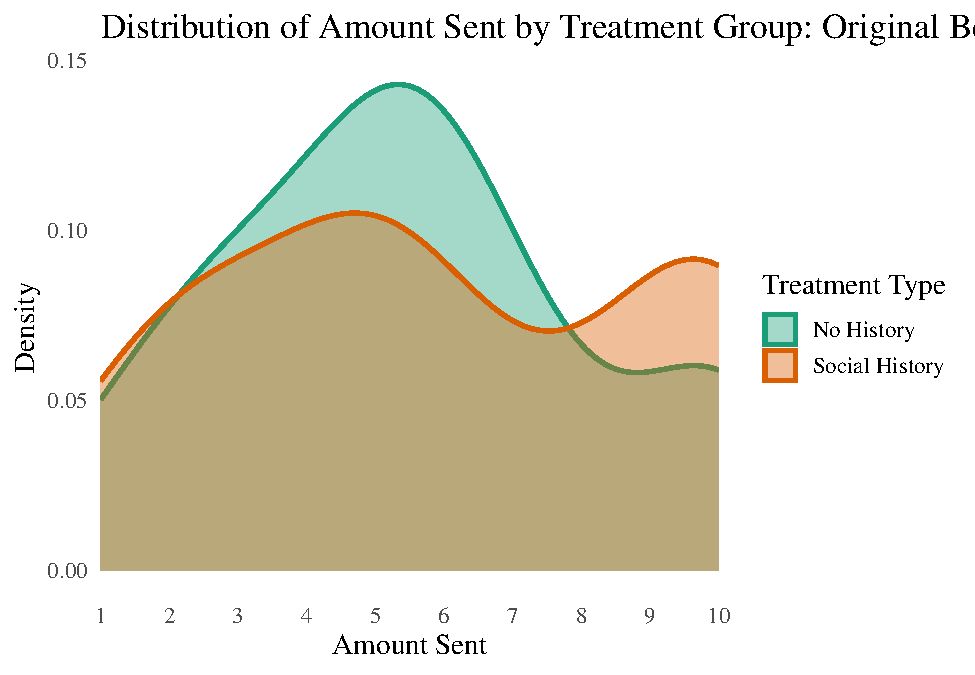
\includegraphics[keepaspectratio]{TrustOverRiskSimualtions_files/figure-latex/0-1.pdf}}

\begin{Shaded}
\begin{Highlighting}[]
\CommentTok{\# Perform Wilcoxon rank{-}sum test (Mann{-}Whitney U) to compare amount sent between groups}
\NormalTok{wilcox\_test\_result }\OtherTok{\textless{}{-}} \FunctionTok{wilcox.exact}\NormalTok{(sent }\SpecialCharTok{\textasciitilde{}}\NormalTok{ treatment, }\AttributeTok{data =}\NormalTok{ berg\_1995, }\AttributeTok{alternative =} \StringTok{"two.sided"}\NormalTok{ )}
\NormalTok{t\_test\_result }\OtherTok{\textless{}{-}} \FunctionTok{t.test}\NormalTok{(sent }\SpecialCharTok{\textasciitilde{}}\NormalTok{ treatment, }\AttributeTok{data =}\NormalTok{ berg\_1995, }\AttributeTok{alternative =} \StringTok{"greater"}\NormalTok{)}
\CommentTok{\# Check what is that we are tresting here}
\NormalTok{group0 }\OtherTok{\textless{}{-}}\NormalTok{ berg\_1995}\SpecialCharTok{$}\NormalTok{sent[}
\NormalTok{  berg\_1995}\SpecialCharTok{$}\NormalTok{treatment }\SpecialCharTok{==} \DecValTok{0}
\NormalTok{]}
\NormalTok{group2 }\OtherTok{\textless{}{-}}\NormalTok{ berg\_1995}\SpecialCharTok{$}\NormalTok{sent[}
\NormalTok{  berg\_1995}\SpecialCharTok{$}\NormalTok{treatment }\SpecialCharTok{==} \DecValTok{1}
\NormalTok{]}
\ControlFlowTok{if}\NormalTok{ (}\FunctionTok{length}\NormalTok{(group0) }\SpecialCharTok{\textgreater{}} \DecValTok{0} \SpecialCharTok{\&\&} \FunctionTok{length}\NormalTok{(group2) }\SpecialCharTok{\textgreater{}} \DecValTok{0}\NormalTok{) \{}
\NormalTok{  si\_test\_result }\OtherTok{\textless{}{-}} \FunctionTok{si.test}\NormalTok{(group0, group2)}
\NormalTok{\} }\ControlFlowTok{else}\NormalTok{ \{}
\NormalTok{  si\_test\_result }\OtherTok{\textless{}{-}} \ConstantTok{NA}
\NormalTok{\}}

\CommentTok{\# Print results of Wilcoxon and t{-}test in an organized way}
\CommentTok{\# Create a data frame with the main results for LaTeX table}
\NormalTok{results\_table }\OtherTok{\textless{}{-}} \FunctionTok{data.frame}\NormalTok{(}
  \AttributeTok{Test =} \FunctionTok{c}\NormalTok{(}\StringTok{"Wilcoxon Exact"}\NormalTok{, }\StringTok{"T{-}Test"}\NormalTok{, }\StringTok{"Stochastic Inequality"}\NormalTok{),}
  \AttributeTok{Statistic =} \FunctionTok{c}\NormalTok{(}
    \FunctionTok{round}\NormalTok{(wilcox\_test\_result}\SpecialCharTok{$}\NormalTok{statistic, }\DecValTok{3}\NormalTok{),}
    \FunctionTok{round}\NormalTok{(t\_test\_result}\SpecialCharTok{$}\NormalTok{statistic, }\DecValTok{3}\NormalTok{),}
    \ControlFlowTok{if}\NormalTok{ (}\SpecialCharTok{!}\FunctionTok{is.null}\NormalTok{(si\_test\_result}\SpecialCharTok{$}\NormalTok{statistic)) }\FunctionTok{round}\NormalTok{(si\_test\_result}\SpecialCharTok{$}\NormalTok{statistic, }\DecValTok{3}\NormalTok{) }\ControlFlowTok{else} \ConstantTok{NA}
\NormalTok{  ),}
  \AttributeTok{P\_Value =} \FunctionTok{c}\NormalTok{(}
    \FunctionTok{signif}\NormalTok{(wilcox\_test\_result}\SpecialCharTok{$}\NormalTok{p.value, }\DecValTok{3}\NormalTok{),}
    \FunctionTok{signif}\NormalTok{(t\_test\_result}\SpecialCharTok{$}\NormalTok{p.value, }\DecValTok{3}\NormalTok{),}
    \ControlFlowTok{if}\NormalTok{ (}\SpecialCharTok{!}\FunctionTok{is.null}\NormalTok{(si\_test\_result}\SpecialCharTok{$}\NormalTok{p.value)) }\FunctionTok{signif}\NormalTok{(si\_test\_result}\SpecialCharTok{$}\NormalTok{p.value, }\DecValTok{3}\NormalTok{) }\ControlFlowTok{else} \ConstantTok{NA}
\NormalTok{  ),}
  \AttributeTok{Alternative =} \FunctionTok{c}\NormalTok{(}
\NormalTok{    wilcox\_test\_result}\SpecialCharTok{$}\NormalTok{alternative,}
\NormalTok{    t\_test\_result}\SpecialCharTok{$}\NormalTok{alternative,}
    \ControlFlowTok{if}\NormalTok{ (}\SpecialCharTok{!}\FunctionTok{is.null}\NormalTok{(si\_test\_result}\SpecialCharTok{$}\NormalTok{alternative)) si\_test\_result}\SpecialCharTok{$}\NormalTok{alternative }\ControlFlowTok{else} \ConstantTok{NA}
\NormalTok{  )}
\NormalTok{)}

\CommentTok{\# Print as LaTeX table}
\NormalTok{knitr}\SpecialCharTok{::}\FunctionTok{kable}\NormalTok{(}
\NormalTok{  results\_table,}
  \AttributeTok{format =} \StringTok{"latex"}\NormalTok{,}
  \AttributeTok{booktabs =} \ConstantTok{TRUE}\NormalTok{,}
  \AttributeTok{caption =} \StringTok{"Summary of Statistical Test Results"}
\NormalTok{)}
\end{Highlighting}
\end{Shaded}

\begin{table}

\caption{\label{tab:0}Summary of Statistical Test Results}
\centering
\begin{tabular}[t]{llrrl}
\toprule
  & Test & Statistic & P\_Value & Alternative\\
\midrule
W & Wilcoxon Exact & 444.000 & 0.956 & two.sided\\
t & T-Test & -0.238 & 0.593 & greater\\
 & Stochastic Inequality & NA & 1.000 & two.sided\\
\bottomrule
\end{tabular}
\end{table}

\section{Simulations of the Trust
Game}\label{simulations-of-the-trust-game}

\subsection{1.1 Size}\label{size}

We ran 1000 simulations for the treatment and the control group to
evaluate the power of the tests. In other words, if our treatment and
control were to generate a sample from the same distribution. (Knowing
that there is no evidence agains the null hypothesis, that they come
from the same distribution). We would expect that on average in less tha
5\% of the cases, we will find evidence to reject the null hypothesis,
meaning that the p-values are greater than 0.05. (All our tests have the
same level)

\begin{Shaded}
\begin{Highlighting}[]
\CommentTok{\#  SIMULATION 1}

\NormalTok{reps }\OtherTok{\textless{}{-}} \DecValTok{1000}
\NormalTok{n }\OtherTok{\textless{}{-}} \DecValTok{100}

\CommentTok{\# File paths for cached results}
\NormalTok{t\_pvalues\_file }\OtherTok{\textless{}{-}} \StringTok{"t\_pvalues\_sim1.rds"}
\NormalTok{wilcox\_pvalues\_file }\OtherTok{\textless{}{-}} \StringTok{"wilcox\_pvalues\_sim1.rds"}

\CommentTok{\# Check if cached results exist}
\ControlFlowTok{if}\NormalTok{ (}\FunctionTok{file.exists}\NormalTok{(t\_pvalues\_file) }\SpecialCharTok{\&\&} \FunctionTok{file.exists}\NormalTok{(wilcox\_pvalues\_file)) \{}
\NormalTok{  t\_pvalues }\OtherTok{\textless{}{-}} \FunctionTok{readRDS}\NormalTok{(t\_pvalues\_file)}
\NormalTok{  wilcox\_exact\_pvalues }\OtherTok{\textless{}{-}} \FunctionTok{readRDS}\NormalTok{(wilcox\_pvalues\_file)}
\NormalTok{\} }\ControlFlowTok{else}\NormalTok{ \{}
\NormalTok{  t\_pvalues }\OtherTok{\textless{}{-}} \FunctionTok{numeric}\NormalTok{(reps)}
\NormalTok{  wilcox\_exact\_pvalues }\OtherTok{\textless{}{-}} \FunctionTok{numeric}\NormalTok{(reps)}
  \ControlFlowTok{for}\NormalTok{ (i }\ControlFlowTok{in} \DecValTok{1}\SpecialCharTok{:}\NormalTok{reps) \{}
\NormalTok{    control }\OtherTok{\textless{}{-}} \FunctionTok{sample}\NormalTok{(berg\_1995}\SpecialCharTok{$}\NormalTok{sent[berg\_1995}\SpecialCharTok{$}\NormalTok{treatment }\SpecialCharTok{==} \DecValTok{0}\NormalTok{], }\AttributeTok{size =}\NormalTok{ n, }\AttributeTok{replace =} \ConstantTok{TRUE}\NormalTok{)}
\NormalTok{    treatment }\OtherTok{\textless{}{-}} \FunctionTok{sample}\NormalTok{(berg\_1995}\SpecialCharTok{$}\NormalTok{sent[berg\_1995}\SpecialCharTok{$}\NormalTok{treatment }\SpecialCharTok{==} \DecValTok{1}\NormalTok{], }\AttributeTok{size =}\NormalTok{ n, }\AttributeTok{replace =} \ConstantTok{TRUE}\NormalTok{)}
\NormalTok{    t\_pvalues[i] }\OtherTok{\textless{}{-}} \FunctionTok{t.test}\NormalTok{(control, treatment)}\SpecialCharTok{$}\NormalTok{p.value}
\NormalTok{    wilcox\_exact\_pvalues[i] }\OtherTok{\textless{}{-}} \FunctionTok{wilcox.exact}\NormalTok{(control, treatment)}\SpecialCharTok{$}\NormalTok{p.value}
\NormalTok{  \}}
  \FunctionTok{saveRDS}\NormalTok{(t\_pvalues, t\_pvalues\_file)}
  \FunctionTok{saveRDS}\NormalTok{(wilcox\_exact\_pvalues, wilcox\_pvalues\_file)}
\NormalTok{\}}

\NormalTok{t\_test\_power }\OtherTok{\textless{}{-}} \FunctionTok{mean}\NormalTok{(t\_pvalues }\SpecialCharTok{\textless{}} \FloatTok{0.05}\NormalTok{)}
\NormalTok{wilcox\_power }\OtherTok{\textless{}{-}} \FunctionTok{mean}\NormalTok{(wilcox\_exact\_pvalues }\SpecialCharTok{\textless{}} \FloatTok{0.05}\NormalTok{)}

\CommentTok{\# Create results table}
\NormalTok{power\_table }\OtherTok{\textless{}{-}} \FunctionTok{data.frame}\NormalTok{(}
  \AttributeTok{Test =} \FunctionTok{c}\NormalTok{(}\StringTok{"t{-}test"}\NormalTok{, }\StringTok{"Wilcoxon Exact"}\NormalTok{),}
  \AttributeTok{Power =} \FunctionTok{c}\NormalTok{(}\FunctionTok{round}\NormalTok{(t\_test\_power, }\DecValTok{3}\NormalTok{), }\FunctionTok{round}\NormalTok{(wilcox\_power, }\DecValTok{3}\NormalTok{))}
\NormalTok{)}

\CommentTok{\# Print as LaTeX table}
\NormalTok{knitr}\SpecialCharTok{::}\FunctionTok{kable}\NormalTok{(}
\NormalTok{  power\_table,}
  \AttributeTok{format =} \StringTok{"latex"}\NormalTok{,}
  \AttributeTok{booktabs =} \ConstantTok{TRUE}\NormalTok{,}
  \AttributeTok{caption =} \StringTok{"Estimated Power for t{-}test and Wilcoxon Test (p{-}value \textless{} 0.05)"}
\NormalTok{)}
\end{Highlighting}
\end{Shaded}

\begin{table}

\caption{\label{tab:1}Estimated Power for t-test and Wilcoxon Test (p-value < 0.05)}
\centering
\begin{tabular}[t]{lr}
\toprule
Test & Power\\
\midrule
t-test & 0.075\\
Wilcoxon Exact & 0.055\\
\bottomrule
\end{tabular}
\end{table}

\subsection{1.2 Power}\label{power}

Now, assuming that the treatment indeed came from a different
distribution, that gives the following probabilities of sending
different amounts, so that:

weights\_llms \textless- c( ``0'' = 0.03, ``1'' = 0.04, ``2'' = 0.05,
``3'' = 0.6, ``4'' = 0.07, ``5'' = 0.25, ``6'' = 0.5, ``7'' = 0.025,
``8'' = 0.1, ``9'' = 0.025, ``10'' = 0.3 )

We are exharcebating the effects observed in Berg (1995) treatment, so
that the treatment group is more likely to send 6, and 10, and less
likely to send 1, compared to the control group. By sampling from such
distribution we will know in advance that under the alternative
hypothesis, we will find a significant difference between the two
groups, and we can estimate the power of the tests under the alternative
hypothesis. We start by running the simulation once and observe the
results of the tests, and then we will run the simulations for different
sample sizes, to estimate the power of the tests under the alternative
hypothesis.

\begin{Shaded}
\begin{Highlighting}[]
\CommentTok{\# SIMULATION 2}

\CommentTok{\# File paths for cached results}
\NormalTok{llm\_means\_file }\OtherTok{\textless{}{-}} \StringTok{"means\_mat\_llm\_sim2.rds"}
\NormalTok{llm\_medians\_file }\OtherTok{\textless{}{-}} \StringTok{"medians\_mat\_llm\_sim2.rds"}
\NormalTok{llm\_t\_pvalues\_file }\OtherTok{\textless{}{-}} \StringTok{"t\_pvalues\_llm\_sim2.rds"}
\NormalTok{llm\_wilcox\_pvalues\_file }\OtherTok{\textless{}{-}} \StringTok{"wilcox\_pvalues\_llm\_sim2.rds"}
\NormalTok{llm\_si\_pvalues\_file }\OtherTok{\textless{}{-}} \StringTok{"si\_pvalues\_llm\_sim2.rds"}

\CommentTok{\# Compute frequency probabilities for each group in berg\_1995$sent}
\NormalTok{sent\_no\_treatment }\OtherTok{\textless{}{-}}\NormalTok{ berg\_1995}\SpecialCharTok{$}\NormalTok{sent[berg\_1995}\SpecialCharTok{$}\NormalTok{treatment }\SpecialCharTok{==} \DecValTok{0}\NormalTok{]}
\NormalTok{sent\_social\_treatment }\OtherTok{\textless{}{-}}\NormalTok{ berg\_1995}\SpecialCharTok{$}\NormalTok{sent[berg\_1995}\SpecialCharTok{$}\NormalTok{treatment }\SpecialCharTok{==} \DecValTok{1}\NormalTok{]}

\CommentTok{\# Get unique values}
\NormalTok{unique\_sent }\OtherTok{\textless{}{-}} \FunctionTok{sort}\NormalTok{(}\FunctionTok{unique}\NormalTok{(berg\_1995}\SpecialCharTok{$}\NormalTok{sent))}

\CommentTok{\# Compute probabilities for each value in each group}
\NormalTok{weights\_no\_treatment }\OtherTok{\textless{}{-}} \FunctionTok{round}\NormalTok{(}\FunctionTok{as.numeric}\NormalTok{(}\FunctionTok{table}\NormalTok{(}\FunctionTok{factor}\NormalTok{(sent\_no\_treatment, }\AttributeTok{levels =}\NormalTok{ unique\_sent)) }\SpecialCharTok{/} \FunctionTok{length}\NormalTok{(berg\_1995}\SpecialCharTok{$}\NormalTok{sent[berg\_1995}\SpecialCharTok{$}\NormalTok{treatment }\SpecialCharTok{==} \DecValTok{0}\NormalTok{])), }\DecValTok{2}\NormalTok{)}
\NormalTok{weights\_social\_treatment }\OtherTok{\textless{}{-}} \FunctionTok{round}\NormalTok{(}\FunctionTok{as.numeric}\NormalTok{(}\FunctionTok{table}\NormalTok{(}\FunctionTok{factor}\NormalTok{(sent\_social\_treatment, }\AttributeTok{levels =}\NormalTok{ unique\_sent)) }\SpecialCharTok{/} \FunctionTok{length}\NormalTok{(berg\_1995}\SpecialCharTok{$}\NormalTok{sent[berg\_1995}\SpecialCharTok{$}\NormalTok{treatment }\SpecialCharTok{==} \DecValTok{1}\NormalTok{])), }\DecValTok{2}\NormalTok{)}

\NormalTok{weights\_db }\OtherTok{\textless{}{-}} \FunctionTok{data.frame}\NormalTok{(}
  \AttributeTok{sent =}\NormalTok{ unique\_sent,}
  \AttributeTok{weight\_no\_treatment =}\NormalTok{ weights\_no\_treatment,}
  \AttributeTok{weight\_social\_treatment =}\NormalTok{ weights\_social\_treatment}
\NormalTok{)}

\CommentTok{\# Participants in the Treatment condition in Berg\textquotesingle{}s experiment were more likely to send 10, and less likely to send 1, compared to the control group.}

\FunctionTok{print}\NormalTok{(weights\_no\_treatment)}
\end{Highlighting}
\end{Shaded}

\begin{verbatim}
##  [1] 0.06 0.06 0.06 0.12 0.06 0.19 0.16 0.09 0.03 0.00 0.16
\end{verbatim}

\begin{Shaded}
\begin{Highlighting}[]
\FunctionTok{print}\NormalTok{(weights\_social\_treatment)}
\end{Highlighting}
\end{Shaded}

\begin{verbatim}
##  [1] 0.11 0.04 0.14 0.07 0.00 0.25 0.04 0.04 0.04 0.04 0.25
\end{verbatim}

\begin{Shaded}
\begin{Highlighting}[]
\CommentTok{\# Assuming that the effect on our treatment will increase the probability of giving 6 , and 10, and reduce the probability}
\CommentTok{\# of giving 1, we can create a vector of weights that will reflect this.}

\NormalTok{weights\_llms }\OtherTok{\textless{}{-}} \FunctionTok{c}\NormalTok{(}\FloatTok{0.03}\NormalTok{, }\FloatTok{0.04}\NormalTok{, }\FloatTok{0.05}\NormalTok{, }\FloatTok{0.6}\NormalTok{, }\FloatTok{0.07}\NormalTok{, }\FloatTok{0.25}\NormalTok{, }\FloatTok{0.5}\NormalTok{, }\FloatTok{0.025}\NormalTok{, }\FloatTok{0.1}\NormalTok{, }\FloatTok{0.025}\NormalTok{, }\FloatTok{0.3}\NormalTok{)}

\NormalTok{treatment\_llms }\OtherTok{\textless{}{-}} \FunctionTok{sample}\NormalTok{(}
\NormalTok{  unique\_sent,}
  \AttributeTok{size =} \FunctionTok{dim}\NormalTok{(berg\_1995[berg\_1995}\SpecialCharTok{$}\NormalTok{treatment }\SpecialCharTok{==} \DecValTok{0}\NormalTok{, ])[}\DecValTok{1}\NormalTok{],}
  \AttributeTok{replace =} \ConstantTok{TRUE}\NormalTok{,}
  \AttributeTok{prob =}\NormalTok{ weights\_llms}
\NormalTok{)}

\CommentTok{\# Adding to the data frame, and testing for possible effects, with the distribution above.}

\NormalTok{berg\_1995\_v1 }\OtherTok{\textless{}{-}} \FunctionTok{rbind}\NormalTok{(}
\NormalTok{  berg\_1995,}
  \FunctionTok{data.frame}\NormalTok{(}
    \AttributeTok{treatment =} \FunctionTok{rep}\NormalTok{(}\DecValTok{2}\NormalTok{, }\FunctionTok{dim}\NormalTok{(berg\_1995[berg\_1995}\SpecialCharTok{$}\NormalTok{treatment }\SpecialCharTok{==} \DecValTok{0}\NormalTok{, ])[}\DecValTok{1}\NormalTok{]),}
    \AttributeTok{sent =}\NormalTok{ treatment\_llms,}
    \AttributeTok{sent\_back =} \ConstantTok{NA}  \CommentTok{\# Assuming no response for the treatment group}
\NormalTok{  )}
\NormalTok{)}

\NormalTok{berg\_1995\_fake\_llm\_treatment }\OtherTok{\textless{}{-}}\NormalTok{ berg\_1995\_v1[berg\_1995\_v1}\SpecialCharTok{$}\NormalTok{treatment }\SpecialCharTok{!=} \DecValTok{1}\NormalTok{, ]}


\FunctionTok{ggplot}\NormalTok{(}
\NormalTok{  berg\_1995\_fake\_llm\_treatment,}
  \FunctionTok{aes}\NormalTok{(}
  \AttributeTok{x =}\NormalTok{ sent,}
  \AttributeTok{fill =} \FunctionTok{factor}\NormalTok{(}
\NormalTok{    treatment,}
    \AttributeTok{labels =} \FunctionTok{c}\NormalTok{(}\StringTok{"Baseline"}\NormalTok{, }\StringTok{"LLMs"}\NormalTok{)}
\NormalTok{  ),}
  \AttributeTok{color =} \FunctionTok{factor}\NormalTok{(}
\NormalTok{    treatment,}
    \AttributeTok{labels =} \FunctionTok{c}\NormalTok{(}\StringTok{"Baseline"}\NormalTok{, }\StringTok{"LLMs"}\NormalTok{)}
\NormalTok{  )}
\NormalTok{  )}
\NormalTok{) }\SpecialCharTok{+}
  \FunctionTok{geom\_density}\NormalTok{(}\AttributeTok{alpha =} \FloatTok{0.4}\NormalTok{, }\AttributeTok{size =} \DecValTok{1}\NormalTok{) }\SpecialCharTok{+}
  \FunctionTok{scale\_fill\_manual}\NormalTok{(}\AttributeTok{values =}\NormalTok{ palette) }\SpecialCharTok{+}
  \FunctionTok{scale\_color\_manual}\NormalTok{(}\AttributeTok{values =}\NormalTok{ palette) }\SpecialCharTok{+}
  \FunctionTok{scale\_x\_continuous}\NormalTok{(}
  \AttributeTok{breaks =} \DecValTok{1}\SpecialCharTok{:}\DecValTok{10}\NormalTok{,}
  \AttributeTok{limits =} \FunctionTok{c}\NormalTok{(}\DecValTok{1}\NormalTok{, }\DecValTok{10}\NormalTok{),}
  \AttributeTok{expand =} \FunctionTok{c}\NormalTok{(}\DecValTok{0}\NormalTok{, }\DecValTok{0}\NormalTok{)}
\NormalTok{  ) }\SpecialCharTok{+}
  \FunctionTok{labs}\NormalTok{(}
  \AttributeTok{title =} \StringTok{"Distribution of Amount Sent: (Simulated Treatment Effects)"}\NormalTok{,}
  \AttributeTok{x =} \StringTok{"Amount Sent"}\NormalTok{,}
  \AttributeTok{y =} \StringTok{"Density"}\NormalTok{,}
  \AttributeTok{fill =} \StringTok{"Treatment Type"}\NormalTok{,}
  \AttributeTok{color =} \StringTok{"Treatment Type"}
\NormalTok{  ) }\SpecialCharTok{+}
\FunctionTok{theme\_minimal}\NormalTok{(}\AttributeTok{base\_size =} \DecValTok{14}\NormalTok{) }\SpecialCharTok{+} \FunctionTok{theme}\NormalTok{(}\AttributeTok{panel.grid =} \FunctionTok{element\_blank}\NormalTok{())}
\end{Highlighting}
\end{Shaded}

\pandocbounded{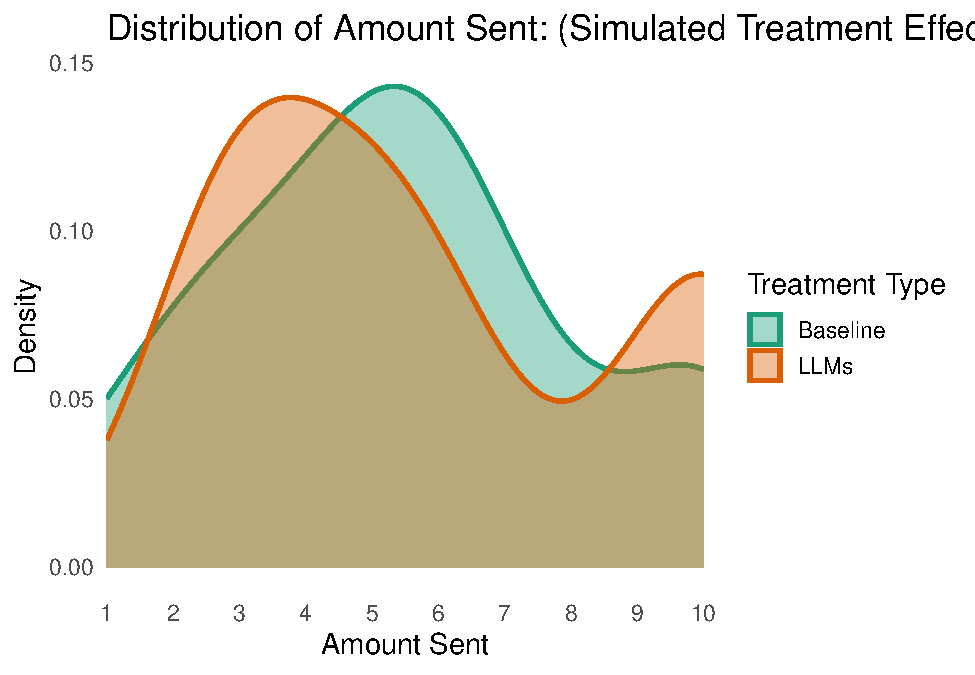
\includegraphics[keepaspectratio]{TrustOverRiskSimualtions_files/figure-latex/2-1.pdf}}

\begin{Shaded}
\begin{Highlighting}[]
\NormalTok{wilcox\_test\_result }\OtherTok{\textless{}{-}} \FunctionTok{wilcox.exact}\NormalTok{(sent }\SpecialCharTok{\textasciitilde{}}\NormalTok{ treatment, }\AttributeTok{data =}\NormalTok{ berg\_1995\_fake\_llm\_treatment, }\AttributeTok{alternative =} \StringTok{"two.sided"}\NormalTok{)}
\NormalTok{t\_test\_result }\OtherTok{\textless{}{-}} \FunctionTok{t.test}\NormalTok{(sent }\SpecialCharTok{\textasciitilde{}}\NormalTok{ treatment, }\AttributeTok{data =}\NormalTok{ berg\_1995\_fake\_llm\_treatment, }\AttributeTok{alternative =} \StringTok{"two.sided"}\NormalTok{)}

\FunctionTok{print}\NormalTok{(wilcox\_test\_result)}
\end{Highlighting}
\end{Shaded}

\begin{verbatim}
## 
##  Exact Wilcoxon rank sum test
## 
## data:  sent by treatment
## W = 466, p-value = 0.5352
## alternative hypothesis: true mu is not equal to 0
\end{verbatim}

\begin{Shaded}
\begin{Highlighting}[]
\FunctionTok{print}\NormalTok{(t\_test\_result)}
\end{Highlighting}
\end{Shaded}

\begin{verbatim}
## 
##  Welch Two Sample t-test
## 
## data:  sent by treatment
## t = -0.94196, df = 61.986, p-value = 0.3499
## alternative hypothesis: true difference in means between group 0 and group 2 is not equal to 0
## 95 percent confidence interval:
##  -2.1464808  0.7714808
## sample estimates:
## mean in group 0 mean in group 2 
##         5.15625         5.84375
\end{verbatim}

\begin{Shaded}
\begin{Highlighting}[]
\CommentTok{\# Power Results for each test }
\CommentTok{\# Power analysis for t{-}test, Wilcoxon, and Stochastic Inequality test using the simulated LLM treatment}

\ControlFlowTok{if}\NormalTok{ (}
  \FunctionTok{file.exists}\NormalTok{(llm\_t\_pvalues\_file) }\SpecialCharTok{\&\&}
  \FunctionTok{file.exists}\NormalTok{(llm\_wilcox\_pvalues\_file) }\SpecialCharTok{\&\&}
  \FunctionTok{file.exists}\NormalTok{(llm\_si\_pvalues\_file) }\SpecialCharTok{\&\&}
  \FunctionTok{file.exists}\NormalTok{(llm\_means\_file) }\SpecialCharTok{\&\&}
  \FunctionTok{file.exists}\NormalTok{(llm\_medians\_file)}
\NormalTok{) \{}
\NormalTok{  t\_pvalues }\OtherTok{\textless{}{-}} \FunctionTok{readRDS}\NormalTok{(llm\_t\_pvalues\_file)}
\NormalTok{  wilcox\_pvalues }\OtherTok{\textless{}{-}} \FunctionTok{readRDS}\NormalTok{(llm\_wilcox\_pvalues\_file)}
\NormalTok{  si\_pvalues }\OtherTok{\textless{}{-}} \FunctionTok{readRDS}\NormalTok{(llm\_si\_pvalues\_file)}
\NormalTok{  means\_mat }\OtherTok{\textless{}{-}} \FunctionTok{readRDS}\NormalTok{(llm\_means\_file)}
\NormalTok{  medians\_mat }\OtherTok{\textless{}{-}} \FunctionTok{readRDS}\NormalTok{(llm\_medians\_file)}
\NormalTok{\} }\ControlFlowTok{else}\NormalTok{ \{}
\NormalTok{  t\_pvalues }\OtherTok{\textless{}{-}} \FunctionTok{numeric}\NormalTok{(reps)}
\NormalTok{  wilcox\_pvalues }\OtherTok{\textless{}{-}} \FunctionTok{numeric}\NormalTok{(reps)}
\NormalTok{  si\_pvalues }\OtherTok{\textless{}{-}} \FunctionTok{numeric}\NormalTok{(reps)}
\NormalTok{  means\_mat }\OtherTok{\textless{}{-}} \FunctionTok{matrix}\NormalTok{(}\ConstantTok{NA}\NormalTok{, }\AttributeTok{nrow =}\NormalTok{ reps, }\AttributeTok{ncol =} \DecValTok{2}\NormalTok{)}
\NormalTok{  medians\_mat }\OtherTok{\textless{}{-}} \FunctionTok{matrix}\NormalTok{(}\ConstantTok{NA}\NormalTok{, }\AttributeTok{nrow =}\NormalTok{ reps, }\AttributeTok{ncol =} \DecValTok{2}\NormalTok{)}

\NormalTok{  pb }\OtherTok{\textless{}{-}}\NormalTok{ progress\_bar}\SpecialCharTok{$}\FunctionTok{new}\NormalTok{(}
  \AttributeTok{format =} \StringTok{"  Simulating [:bar] :percent eta: :eta"}\NormalTok{,}
  \AttributeTok{total =}\NormalTok{ reps, }\AttributeTok{clear =} \ConstantTok{FALSE}\NormalTok{, }\AttributeTok{width =} \DecValTok{60}
\NormalTok{  )}

  \ControlFlowTok{for}\NormalTok{ (i }\ControlFlowTok{in} \DecValTok{1}\SpecialCharTok{:}\NormalTok{reps) \{}
\NormalTok{  control }\OtherTok{\textless{}{-}} \FunctionTok{sample}\NormalTok{(berg\_1995}\SpecialCharTok{$}\NormalTok{sent[berg\_1995}\SpecialCharTok{$}\NormalTok{treatment }\SpecialCharTok{==} \DecValTok{0}\NormalTok{], }\AttributeTok{size =}\NormalTok{ n, }\AttributeTok{replace =} \ConstantTok{TRUE}\NormalTok{)}
\NormalTok{  treatment }\OtherTok{\textless{}{-}} \FunctionTok{sample}\NormalTok{(unique\_sent, }\AttributeTok{size =}\NormalTok{ n, }\AttributeTok{replace =} \ConstantTok{TRUE}\NormalTok{, }\AttributeTok{prob =}\NormalTok{ weights\_llms)}
  
  \CommentTok{\# t{-}test}
\NormalTok{  t\_pvalues[i] }\OtherTok{\textless{}{-}} \FunctionTok{t.test}\NormalTok{(control, treatment)}\SpecialCharTok{$}\NormalTok{p.value}
  
  \CommentTok{\# Wilcoxon exact test}
\NormalTok{  wilcox\_pvalues[i] }\OtherTok{\textless{}{-}} \FunctionTok{wilcox.exact}\NormalTok{(control, treatment)}\SpecialCharTok{$}\NormalTok{p.value}
  
  \CommentTok{\# Stochastic Inequality test}
\NormalTok{  si\_res }\OtherTok{\textless{}{-}} \FunctionTok{si.test}\NormalTok{(control, treatment)}
\NormalTok{  si\_pvalues[i] }\OtherTok{\textless{}{-}} \ControlFlowTok{if}\NormalTok{ (}\SpecialCharTok{!}\FunctionTok{is.null}\NormalTok{(si\_res}\SpecialCharTok{$}\NormalTok{p.value)) si\_res}\SpecialCharTok{$}\NormalTok{p.value }\ControlFlowTok{else} \ConstantTok{NA}

  \CommentTok{\# Store means and medians for this simulation}
\NormalTok{  means\_mat[i, ] }\OtherTok{\textless{}{-}} \FunctionTok{c}\NormalTok{(}\FunctionTok{mean}\NormalTok{(control), }\FunctionTok{mean}\NormalTok{(treatment))}
\NormalTok{  medians\_mat[i, ] }\OtherTok{\textless{}{-}} \FunctionTok{c}\NormalTok{(}\FunctionTok{median}\NormalTok{(control), }\FunctionTok{median}\NormalTok{(treatment))}
  
\NormalTok{  pb}\SpecialCharTok{$}\FunctionTok{tick}\NormalTok{()}
\NormalTok{  \}}

  \FunctionTok{saveRDS}\NormalTok{(t\_pvalues, llm\_t\_pvalues\_file)}
  \FunctionTok{saveRDS}\NormalTok{(wilcox\_pvalues, llm\_wilcox\_pvalues\_file)}
  \FunctionTok{saveRDS}\NormalTok{(si\_pvalues, llm\_si\_pvalues\_file)}
  \FunctionTok{saveRDS}\NormalTok{(means\_mat, llm\_means\_file)}
  \FunctionTok{saveRDS}\NormalTok{(medians\_mat, llm\_medians\_file)}
\NormalTok{\}}

\CommentTok{\# Compute average means and medians across all simulations}
\NormalTok{summary\_stats }\OtherTok{\textless{}{-}} \FunctionTok{data.frame}\NormalTok{(}
  \AttributeTok{Group =} \FunctionTok{c}\NormalTok{(}\StringTok{"Control"}\NormalTok{, }\StringTok{"LLM Treatment"}\NormalTok{),}
  \AttributeTok{Mean =} \FunctionTok{round}\NormalTok{(}\FunctionTok{colMeans}\NormalTok{(means\_mat, }\AttributeTok{na.rm =} \ConstantTok{TRUE}\NormalTok{), }\DecValTok{3}\NormalTok{),}
  \AttributeTok{Median =} \FunctionTok{round}\NormalTok{(}\FunctionTok{colMeans}\NormalTok{(medians\_mat, }\AttributeTok{na.rm =} \ConstantTok{TRUE}\NormalTok{), }\DecValTok{3}\NormalTok{)}
\NormalTok{)}
\FunctionTok{print}\NormalTok{(summary\_stats)}
\end{Highlighting}
\end{Shaded}

\begin{verbatim}
##           Group  Mean Median
## 1       Control 5.160  5.101
## 2 LLM Treatment 5.359  5.318
\end{verbatim}

\begin{Shaded}
\begin{Highlighting}[]
\CommentTok{\# Transform means\_mat for plotting}
\NormalTok{means\_mat }\OtherTok{\textless{}{-}} \FunctionTok{as.data.frame}\NormalTok{(means\_mat)}
\FunctionTok{colnames}\NormalTok{(means\_mat) }\OtherTok{\textless{}{-}} \FunctionTok{c}\NormalTok{(}\StringTok{"Control"}\NormalTok{, }\StringTok{"LLM\_Treatment"}\NormalTok{)}
\NormalTok{means\_mat\_long }\OtherTok{\textless{}{-}}\NormalTok{ tidyr}\SpecialCharTok{::}\FunctionTok{pivot\_longer}\NormalTok{(}
\NormalTok{  means\_mat,}
  \AttributeTok{cols =} \FunctionTok{everything}\NormalTok{(),}
  \AttributeTok{names\_to =} \StringTok{"group"}\NormalTok{,}
  \AttributeTok{values\_to =} \StringTok{"value"}
\NormalTok{)}

\FunctionTok{library}\NormalTok{(ggplot2)}
\FunctionTok{ggplot}\NormalTok{(means\_mat\_long, }\FunctionTok{aes}\NormalTok{(}\AttributeTok{x =}\NormalTok{ value, }\AttributeTok{fill =}\NormalTok{ group, }\AttributeTok{color =}\NormalTok{ group)) }\SpecialCharTok{+}
  \FunctionTok{geom\_density}\NormalTok{(}\AttributeTok{alpha =} \FloatTok{0.4}\NormalTok{, }\AttributeTok{size =} \DecValTok{1}\NormalTok{) }\SpecialCharTok{+}
  \FunctionTok{scale\_fill\_manual}\NormalTok{(}\AttributeTok{values =} \FunctionTok{c}\NormalTok{(}\StringTok{"\#1b9e77"}\NormalTok{, }\StringTok{"\#d95f02"}\NormalTok{)) }\SpecialCharTok{+}
  \FunctionTok{scale\_color\_manual}\NormalTok{(}\AttributeTok{values =} \FunctionTok{c}\NormalTok{(}\StringTok{"\#1b9e77"}\NormalTok{, }\StringTok{"\#d95f02"}\NormalTok{)) }\SpecialCharTok{+}
  \FunctionTok{labs}\NormalTok{(}
  \AttributeTok{title =} \StringTok{"Distribution of Amount Mean(Sent): Control vs. LLM Treatment (Simulated)"}\NormalTok{,}
  \AttributeTok{x =} \StringTok{"Amount Sent"}\NormalTok{,}
  \AttributeTok{y =} \StringTok{"Density"}\NormalTok{,}
  \AttributeTok{fill =} \StringTok{"Group"}\NormalTok{,}
  \AttributeTok{color =} \StringTok{"Group"}
\NormalTok{  ) }\SpecialCharTok{+}
  \FunctionTok{theme\_minimal}\NormalTok{(}\AttributeTok{base\_size =} \DecValTok{14}\NormalTok{) }\SpecialCharTok{+}
  \FunctionTok{theme}\NormalTok{(}\AttributeTok{panel.grid =} \FunctionTok{element\_blank}\NormalTok{())}
\end{Highlighting}
\end{Shaded}

\pandocbounded{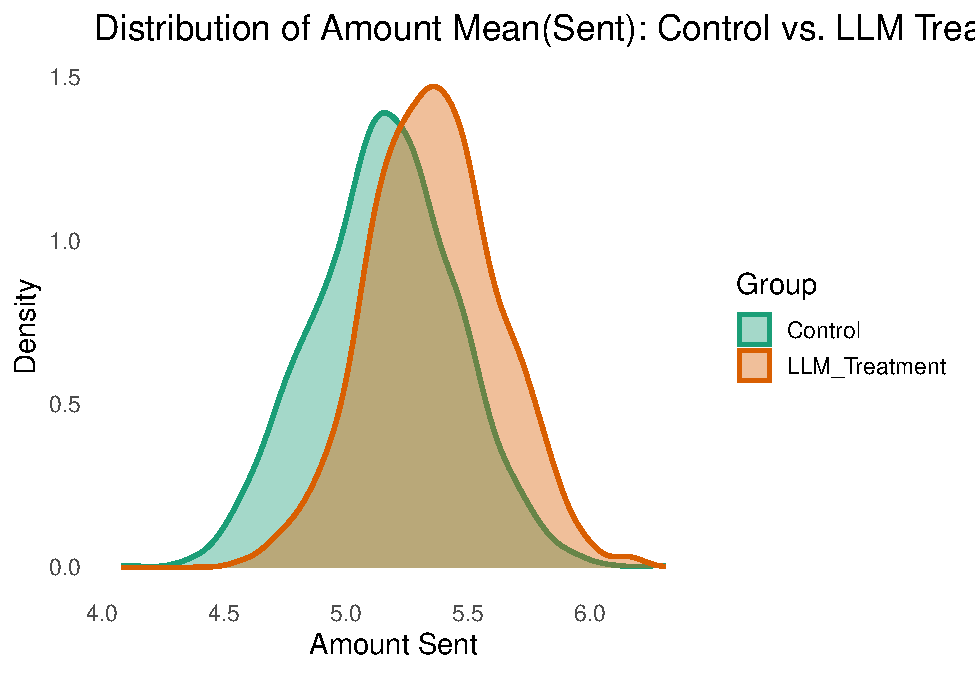
\includegraphics[keepaspectratio]{TrustOverRiskSimualtions_files/figure-latex/2-2.pdf}}

\begin{Shaded}
\begin{Highlighting}[]
\NormalTok{power\_table\_llm }\OtherTok{\textless{}{-}} \FunctionTok{data.frame}\NormalTok{(}
  \AttributeTok{Test =} \FunctionTok{c}\NormalTok{(}\StringTok{"t{-}test"}\NormalTok{, }\StringTok{"Wilcoxon Exact"}\NormalTok{, }\StringTok{"Stochastic Inequality"}\NormalTok{),}
  \AttributeTok{Power =} \FunctionTok{c}\NormalTok{(}
  \FunctionTok{round}\NormalTok{(}\FunctionTok{mean}\NormalTok{(t\_pvalues }\SpecialCharTok{\textless{}} \FloatTok{0.05}\NormalTok{, }\AttributeTok{na.rm =} \ConstantTok{TRUE}\NormalTok{), }\DecValTok{3}\NormalTok{),}
  \FunctionTok{round}\NormalTok{(}\FunctionTok{mean}\NormalTok{(wilcox\_pvalues }\SpecialCharTok{\textless{}} \FloatTok{0.05}\NormalTok{, }\AttributeTok{na.rm =} \ConstantTok{TRUE}\NormalTok{), }\DecValTok{3}\NormalTok{),}
  \FunctionTok{round}\NormalTok{(}\FunctionTok{mean}\NormalTok{(si\_pvalues }\SpecialCharTok{\textless{}} \FloatTok{0.05}\NormalTok{, }\AttributeTok{na.rm =} \ConstantTok{TRUE}\NormalTok{), }\DecValTok{3}\NormalTok{)}
\NormalTok{  )}
\NormalTok{)}

\NormalTok{knitr}\SpecialCharTok{::}\FunctionTok{kable}\NormalTok{(}
\NormalTok{  power\_table\_llm,}
  \AttributeTok{format =} \StringTok{"latex"}\NormalTok{,}
  \AttributeTok{booktabs =} \ConstantTok{TRUE}\NormalTok{,}
  \AttributeTok{caption =} \StringTok{"Estimated Power for t{-}test, Wilcoxon, and Stochastic Inequality Test (Simulated LLM Treatment, p{-}value \textless{} 0.05)"}
\NormalTok{)}
\end{Highlighting}
\end{Shaded}

\begin{table}

\caption{\label{tab:2}Estimated Power for t-test, Wilcoxon, and Stochastic Inequality Test (Simulated LLM Treatment, p-value < 0.05)}
\centering
\begin{tabular}[t]{lr}
\toprule
Test & Power\\
\midrule
t-test & 0.087\\
Wilcoxon Exact & 0.069\\
Stochastic Inequality & 0.023\\
\bottomrule
\end{tabular}
\end{table}

\section{1.3 Power Analysis}\label{power-analysis}

We will now compare the power of the three tests (t-test, Wilcoxon, and
Stochastic Inequality test) to determine how many samples we need to
detect a significant difference between the two groups, assuming the
treatment group has a different distribution of amounts sent.

\begin{Shaded}
\begin{Highlighting}[]
\CommentTok{\# SIMULATION 3}
\CommentTok{\# Define a sequence of n values}
\NormalTok{n\_values }\OtherTok{\textless{}{-}} \FunctionTok{seq}\NormalTok{(}\DecValTok{10}\NormalTok{, }\DecValTok{80}\NormalTok{, }\AttributeTok{by =} \DecValTok{5}\NormalTok{)}

\CommentTok{\# File paths for cached results}
\NormalTok{power\_results\_file }\OtherTok{\textless{}{-}} \StringTok{"power\_results\_sim3.rds"}

\CommentTok{\# Checking if there is any difference in means:}
\CommentTok{\# Difference in means of approximately 0.75 points. (or 7.5\%)}
\FunctionTok{aggregate}\NormalTok{(sent }\SpecialCharTok{\textasciitilde{}}\NormalTok{ treatment, }\AttributeTok{data =}\NormalTok{ berg\_1995, mean)}
\end{Highlighting}
\end{Shaded}

\begin{verbatim}
##   treatment     sent
## 1         0 5.156250
## 2         1 5.357143
\end{verbatim}

\begin{Shaded}
\begin{Highlighting}[]
\ControlFlowTok{if}\NormalTok{ (}\FunctionTok{file.exists}\NormalTok{(power\_results\_file)) \{}
\NormalTok{  power\_results }\OtherTok{\textless{}{-}} \FunctionTok{readRDS}\NormalTok{(power\_results\_file)}
\NormalTok{\} }\ControlFlowTok{else}\NormalTok{ \{}
  \CommentTok{\# Prepare data frame to store results}
\NormalTok{  power\_results }\OtherTok{\textless{}{-}} \FunctionTok{data.frame}\NormalTok{(}
    \AttributeTok{n =} \FunctionTok{integer}\NormalTok{(),}
    \AttributeTok{t\_test\_power =} \FunctionTok{numeric}\NormalTok{(),}
    \AttributeTok{wilcox\_power =} \FunctionTok{numeric}\NormalTok{()}
\NormalTok{  )}

\NormalTok{  pb }\OtherTok{\textless{}{-}}\NormalTok{ progress\_bar}\SpecialCharTok{$}\FunctionTok{new}\NormalTok{(}
    \AttributeTok{format =} \StringTok{"  Simulating [:bar] :percent eta: :eta"}\NormalTok{,}
    \AttributeTok{total =} \FunctionTok{length}\NormalTok{(n\_values), }\AttributeTok{clear =} \ConstantTok{FALSE}\NormalTok{, }\AttributeTok{width =} \DecValTok{60}
\NormalTok{  )}
  \ControlFlowTok{for}\NormalTok{ (n }\ControlFlowTok{in}\NormalTok{ n\_values) \{}
    \CommentTok{\# t{-}test power}
\NormalTok{    t\_pvalues }\OtherTok{\textless{}{-}} \FunctionTok{numeric}\NormalTok{(reps)}
\NormalTok{    w\_pvalues }\OtherTok{\textless{}{-}} \FunctionTok{numeric}\NormalTok{(reps)}
    \ControlFlowTok{for}\NormalTok{ (i }\ControlFlowTok{in} \DecValTok{1}\SpecialCharTok{:}\NormalTok{reps) \{}
\NormalTok{      control }\OtherTok{\textless{}{-}} \FunctionTok{sample}\NormalTok{(berg\_1995}\SpecialCharTok{$}\NormalTok{sent[berg\_1995}\SpecialCharTok{$}\NormalTok{treatment }\SpecialCharTok{==} \DecValTok{0}\NormalTok{], }\AttributeTok{size =}\NormalTok{ n, }\AttributeTok{replace =} \ConstantTok{TRUE}\NormalTok{)}
\NormalTok{      treatment }\OtherTok{\textless{}{-}} \FunctionTok{sample}\NormalTok{(unique\_sent, }\AttributeTok{size =}\NormalTok{ n, }\AttributeTok{replace =} \ConstantTok{TRUE}\NormalTok{, }\AttributeTok{prob =}\NormalTok{ weights\_llms)}
\NormalTok{      t\_pvalues[i] }\OtherTok{\textless{}{-}} \FunctionTok{t.test}\NormalTok{(control, treatment)}\SpecialCharTok{$}\NormalTok{p.value}
\NormalTok{      w\_pvalues[i] }\OtherTok{\textless{}{-}} \FunctionTok{wilcox.exact}\NormalTok{(control, treatment)}\SpecialCharTok{$}\NormalTok{p.value}
\NormalTok{    \}}
\NormalTok{    t\_test\_power }\OtherTok{\textless{}{-}} \FunctionTok{mean}\NormalTok{(t\_pvalues }\SpecialCharTok{\textless{}} \FloatTok{0.05}\NormalTok{)}
\NormalTok{    wilcox\_power }\OtherTok{\textless{}{-}} \FunctionTok{mean}\NormalTok{(w\_pvalues }\SpecialCharTok{\textless{}} \FloatTok{0.05}\NormalTok{)}
    \CommentTok{\# Store results}
\NormalTok{    power\_results }\OtherTok{\textless{}{-}} \FunctionTok{rbind}\NormalTok{(}
\NormalTok{      power\_results,}
      \FunctionTok{data.frame}\NormalTok{(}\AttributeTok{n =}\NormalTok{ n, }\AttributeTok{t\_test\_power =}\NormalTok{ t\_test\_power, }\AttributeTok{wilcox\_power =}\NormalTok{ wilcox\_power)}
\NormalTok{    )}
\NormalTok{    pb}\SpecialCharTok{$}\FunctionTok{tick}\NormalTok{()}
\NormalTok{  \}}
  \FunctionTok{saveRDS}\NormalTok{(power\_results, power\_results\_file)}
\NormalTok{\}}

\CommentTok{\# Reshape for plotting}
\FunctionTok{library}\NormalTok{(tidyr)}
\NormalTok{power\_long }\OtherTok{\textless{}{-}} \FunctionTok{pivot\_longer}\NormalTok{(power\_results, }\AttributeTok{cols =} \FunctionTok{c}\NormalTok{(}\StringTok{"t\_test\_power"}\NormalTok{, }\StringTok{"wilcox\_power"}\NormalTok{),}
                           \AttributeTok{names\_to =} \StringTok{"test"}\NormalTok{, }\AttributeTok{values\_to =} \StringTok{"power"}\NormalTok{)}

\CommentTok{\# Plot}
\FunctionTok{library}\NormalTok{(ggplot2)}
\FunctionTok{ggplot}\NormalTok{(power\_long, }\FunctionTok{aes}\NormalTok{(}\AttributeTok{x =}\NormalTok{ n, }\AttributeTok{y =}\NormalTok{ power, }\AttributeTok{color =}\NormalTok{ test)) }\SpecialCharTok{+}
  \FunctionTok{geom\_line}\NormalTok{(}\AttributeTok{size =} \FloatTok{1.2}\NormalTok{) }\SpecialCharTok{+}
  \FunctionTok{geom\_point}\NormalTok{(}\AttributeTok{size =} \DecValTok{2}\NormalTok{) }\SpecialCharTok{+}
  \FunctionTok{labs}\NormalTok{(}
    \AttributeTok{title =} \StringTok{"Power Curve for t{-}test and Wilcoxon Test"}\NormalTok{,}
    \AttributeTok{x =} \StringTok{"Sample Size (n)"}\NormalTok{,}
    \AttributeTok{y =} \StringTok{"Power (P{-}value \textgreater{} 0.05)"}\NormalTok{,}
    \AttributeTok{color =} \StringTok{"Test"}
\NormalTok{  ) }\SpecialCharTok{+}
  \FunctionTok{scale\_color\_manual}\NormalTok{(}\AttributeTok{values =} \FunctionTok{c}\NormalTok{(}\StringTok{"t\_test\_power"} \OtherTok{=} \StringTok{"\#1b9e77"}\NormalTok{, }\StringTok{"wilcox\_power"} \OtherTok{=} \StringTok{"\#d95f02"}\NormalTok{),}
                     \AttributeTok{labels =} \FunctionTok{c}\NormalTok{(}\StringTok{"t\_test\_power"} \OtherTok{=} \StringTok{"t{-}test"}\NormalTok{, }\StringTok{"wilcox\_power"} \OtherTok{=} \StringTok{"Wilcoxon"}\NormalTok{)) }\SpecialCharTok{+}
  \FunctionTok{theme\_minimal}\NormalTok{(}\AttributeTok{base\_size =} \DecValTok{14}\NormalTok{, }\AttributeTok{base\_family =} \StringTok{"Times"}\NormalTok{) }\SpecialCharTok{+}
  \FunctionTok{theme}\NormalTok{(}\AttributeTok{panel.grid =} \FunctionTok{element\_blank}\NormalTok{())}
\end{Highlighting}
\end{Shaded}

\pandocbounded{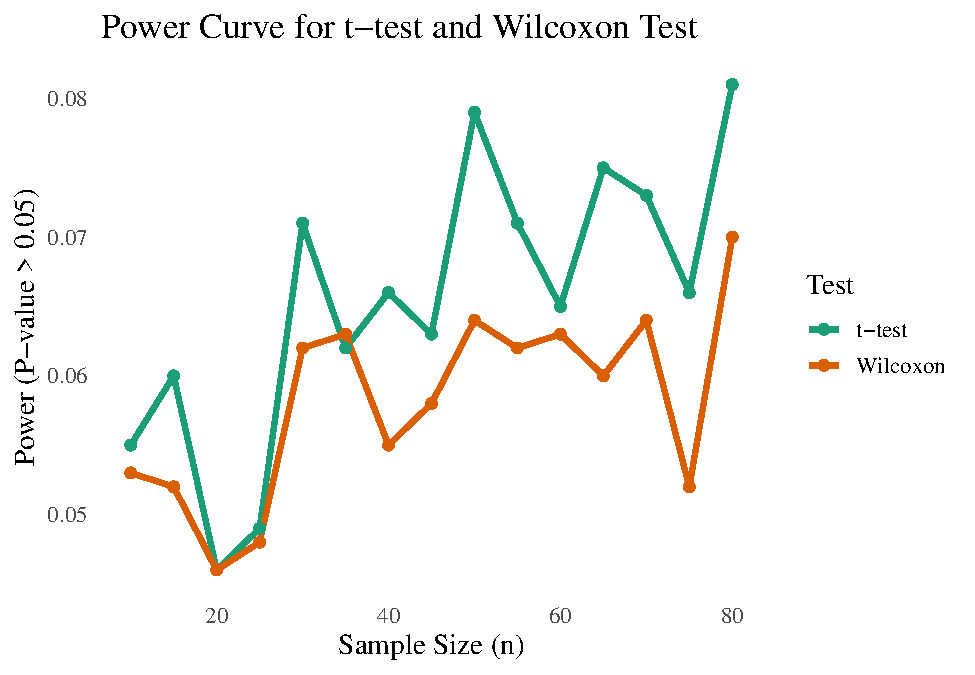
\includegraphics[keepaspectratio]{TrustOverRiskSimualtions_files/figure-latex/3-1.pdf}}

\begin{Shaded}
\begin{Highlighting}[]
\CommentTok{\# Print the power results as a LaTeX table}
\NormalTok{knitr}\SpecialCharTok{::}\FunctionTok{kable}\NormalTok{(}
\NormalTok{  power\_results,}
  \AttributeTok{format =} \StringTok{"latex"}\NormalTok{,}
  \AttributeTok{booktabs =} \ConstantTok{TRUE}\NormalTok{,}
  \AttributeTok{caption =} \StringTok{"Power Results for t{-}test and Wilcoxon Test Across Sample Sizes"}
\NormalTok{)}
\end{Highlighting}
\end{Shaded}

\begin{table}

\caption{\label{tab:3}Power Results for t-test and Wilcoxon Test Across Sample Sizes}
\centering
\begin{tabular}[t]{rrr}
\toprule
n & t\_test\_power & wilcox\_power\\
\midrule
10 & 0.055 & 0.053\\
15 & 0.060 & 0.052\\
20 & 0.046 & 0.046\\
25 & 0.049 & 0.048\\
30 & 0.071 & 0.062\\
\addlinespace
35 & 0.062 & 0.063\\
40 & 0.066 & 0.055\\
45 & 0.063 & 0.058\\
50 & 0.079 & 0.064\\
55 & 0.071 & 0.062\\
\addlinespace
60 & 0.065 & 0.063\\
65 & 0.075 & 0.060\\
70 & 0.073 & 0.064\\
75 & 0.066 & 0.052\\
80 & 0.081 & 0.070\\
\bottomrule
\end{tabular}
\end{table}

\section{1.4 Including Interaction
Effects}\label{including-interaction-effects}

We expect that users that are more familiarized with LLMs, will be more
likely to send higher amounts. We will then simply ask participants to
provide us with their email address with which they are registered in
OpenAI

\begin{Shaded}
\begin{Highlighting}[]
\CommentTok{\# SIMULATION 4}
\CommentTok{\# Simulate interaction: probability of having an LLM account is higher in the treatment group}

\FunctionTok{set.seed}\NormalTok{(}\DecValTok{123}\NormalTok{) }\CommentTok{\# for reproducibility}

\CommentTok{\# File paths for cached results}
\NormalTok{reg\_pvalues\_int\_file }\OtherTok{\textless{}{-}} \StringTok{"reg\_pvalues\_int\_sim4.rds"}
\NormalTok{wilcox\_pvalues\_by\_llm\_file }\OtherTok{\textless{}{-}} \StringTok{"wilcox\_pvalues\_by\_llm\_sim4.rds"}

\ControlFlowTok{if}\NormalTok{ (}\FunctionTok{file.exists}\NormalTok{(reg\_pvalues\_int\_file) }\SpecialCharTok{\&\&} \FunctionTok{file.exists}\NormalTok{(wilcox\_pvalues\_by\_llm\_file)) \{}
\NormalTok{  reg\_pvalues\_int }\OtherTok{\textless{}{-}} \FunctionTok{readRDS}\NormalTok{(reg\_pvalues\_int\_file)}
\NormalTok{  wilcox\_pvalues\_by\_llm }\OtherTok{\textless{}{-}} \FunctionTok{readRDS}\NormalTok{(wilcox\_pvalues\_by\_llm\_file)}
\NormalTok{\} }\ControlFlowTok{else}\NormalTok{ \{}
\NormalTok{  reg\_pvalues\_int }\OtherTok{\textless{}{-}} \FunctionTok{data.frame}\NormalTok{(}
    \AttributeTok{group\_treatment =} \FunctionTok{numeric}\NormalTok{(reps),}
    \AttributeTok{llm\_account =} \FunctionTok{numeric}\NormalTok{(reps),}
    \AttributeTok{interaction =} \FunctionTok{numeric}\NormalTok{(reps)}
\NormalTok{  )}

\NormalTok{  wilcox\_pvalues\_by\_llm }\OtherTok{\textless{}{-}} \FunctionTok{data.frame}\NormalTok{(}
    \AttributeTok{rep =} \DecValTok{1}\SpecialCharTok{:}\NormalTok{reps,}
    \AttributeTok{llm0 =} \ConstantTok{NA\_real\_}\NormalTok{,}
    \AttributeTok{llm1 =} \ConstantTok{NA\_real\_}
\NormalTok{  )}

\NormalTok{  pb }\OtherTok{\textless{}{-}}\NormalTok{ progress\_bar}\SpecialCharTok{$}\FunctionTok{new}\NormalTok{(}
    \AttributeTok{format =} \StringTok{"  Simulating [:bar] :percent eta: :eta"}\NormalTok{,}
    \AttributeTok{total =}\NormalTok{ reps, }\AttributeTok{clear =} \ConstantTok{FALSE}\NormalTok{, }\AttributeTok{width =} \DecValTok{60}
\NormalTok{  )}

  \ControlFlowTok{for}\NormalTok{ (i }\ControlFlowTok{in} \DecValTok{1}\SpecialCharTok{:}\NormalTok{reps) \{}
    \CommentTok{\# Sample control group (baseline)}
\NormalTok{    control\_sent }\OtherTok{\textless{}{-}} \FunctionTok{sample}\NormalTok{(berg\_1995}\SpecialCharTok{$}\NormalTok{sent[berg\_1995}\SpecialCharTok{$}\NormalTok{treatment }\SpecialCharTok{==} \DecValTok{0}\NormalTok{], }\AttributeTok{size =}\NormalTok{ n, }\AttributeTok{replace =} \ConstantTok{TRUE}\NormalTok{)}
    \CommentTok{\# Probability of LLM account increases with sent amount (e.g., logistic or linear scaling)}
\NormalTok{    control\_llm\_prob }\OtherTok{\textless{}{-}}\NormalTok{ scales}\SpecialCharTok{::}\FunctionTok{rescale}\NormalTok{(control\_sent, }\AttributeTok{to =} \FunctionTok{c}\NormalTok{(}\FloatTok{0.2}\NormalTok{, }\FloatTok{0.7}\NormalTok{)) }\CommentTok{\# adjust range as needed}
\NormalTok{    control\_llm\_account }\OtherTok{\textless{}{-}} \FunctionTok{rbinom}\NormalTok{(n, }\DecValTok{1}\NormalTok{, }\AttributeTok{prob =}\NormalTok{ control\_llm\_prob)}

    \CommentTok{\# Sample treatment group (LLM treatment)}
\NormalTok{    treatment\_sent }\OtherTok{\textless{}{-}} \FunctionTok{sample}\NormalTok{(unique\_sent, }\AttributeTok{size =}\NormalTok{ n, }\AttributeTok{replace =} \ConstantTok{TRUE}\NormalTok{, }\AttributeTok{prob =}\NormalTok{ weights\_llms)}
\NormalTok{    treatment\_llm\_prob }\OtherTok{\textless{}{-}}\NormalTok{ scales}\SpecialCharTok{::}\FunctionTok{rescale}\NormalTok{(treatment\_sent, }\AttributeTok{to =} \FunctionTok{c}\NormalTok{(}\FloatTok{0.4}\NormalTok{, }\FloatTok{0.95}\NormalTok{)) }\CommentTok{\# higher base probability}
\NormalTok{    treatment\_llm\_account }\OtherTok{\textless{}{-}} \FunctionTok{rbinom}\NormalTok{(n, }\DecValTok{1}\NormalTok{, }\AttributeTok{prob =}\NormalTok{ treatment\_llm\_prob)}

    \CommentTok{\# Combine into a single data frame}
\NormalTok{    sim\_data }\OtherTok{\textless{}{-}} \FunctionTok{data.frame}\NormalTok{(}
      \AttributeTok{group =} \FunctionTok{rep}\NormalTok{(}\FunctionTok{c}\NormalTok{(}\StringTok{"control"}\NormalTok{, }\StringTok{"treatment"}\NormalTok{), }\AttributeTok{each =}\NormalTok{ n),}
      \AttributeTok{sent =} \FunctionTok{c}\NormalTok{(control\_sent, treatment\_sent),}
      \AttributeTok{llm\_account =} \FunctionTok{c}\NormalTok{(control\_llm\_account, treatment\_llm\_account)}
\NormalTok{    )}

    \CommentTok{\# Fit linear regression: sent \textasciitilde{} group + llm\_account + group:llm\_account}
\NormalTok{    sim\_data}\SpecialCharTok{$}\NormalTok{group }\OtherTok{\textless{}{-}} \FunctionTok{factor}\NormalTok{(sim\_data}\SpecialCharTok{$}\NormalTok{group, }\AttributeTok{levels =} \FunctionTok{c}\NormalTok{(}\StringTok{"control"}\NormalTok{, }\StringTok{"treatment"}\NormalTok{))}
\NormalTok{    fit }\OtherTok{\textless{}{-}} \FunctionTok{lm}\NormalTok{(sent }\SpecialCharTok{\textasciitilde{}}\NormalTok{ group }\SpecialCharTok{+}\NormalTok{ llm\_account }\SpecialCharTok{+}\NormalTok{ group}\SpecialCharTok{:}\NormalTok{llm\_account, }\AttributeTok{data =}\NormalTok{ sim\_data)}
\NormalTok{    reg\_summary }\OtherTok{\textless{}{-}} \FunctionTok{summary}\NormalTok{(fit)}\SpecialCharTok{$}\NormalTok{coefficients}

    \CommentTok{\# Extract p{-}values for group\_treatment, llm\_account, and interaction}
\NormalTok{    reg\_pvalues\_int}\SpecialCharTok{$}\NormalTok{group\_treatment[i] }\OtherTok{\textless{}{-}} \ControlFlowTok{if}\NormalTok{ (}\StringTok{"grouptreatment"} \SpecialCharTok{\%in\%} \FunctionTok{rownames}\NormalTok{(reg\_summary)) reg\_summary[}\StringTok{"grouptreatment"}\NormalTok{, }\StringTok{"Pr(\textgreater{}|t|)"}\NormalTok{] }\ControlFlowTok{else} \ConstantTok{NA}
\NormalTok{    reg\_pvalues\_int}\SpecialCharTok{$}\NormalTok{llm\_account[i] }\OtherTok{\textless{}{-}} \ControlFlowTok{if}\NormalTok{ (}\StringTok{"llm\_account"} \SpecialCharTok{\%in\%} \FunctionTok{rownames}\NormalTok{(reg\_summary)) reg\_summary[}\StringTok{"llm\_account"}\NormalTok{, }\StringTok{"Pr(\textgreater{}|t|)"}\NormalTok{] }\ControlFlowTok{else} \ConstantTok{NA}
\NormalTok{    reg\_pvalues\_int}\SpecialCharTok{$}\NormalTok{interaction[i] }\OtherTok{\textless{}{-}} \ControlFlowTok{if}\NormalTok{ (}\StringTok{"grouptreatment:llm\_account"} \SpecialCharTok{\%in\%} \FunctionTok{rownames}\NormalTok{(reg\_summary)) reg\_summary[}\StringTok{"grouptreatment:llm\_account"}\NormalTok{, }\StringTok{"Pr(\textgreater{}|t|)"}\NormalTok{] }\ControlFlowTok{else} \ConstantTok{NA}

    \CommentTok{\# Wilcoxon test between control and treatment groups, separately for each llm\_account value}
    \ControlFlowTok{for}\NormalTok{ (llm\_val }\ControlFlowTok{in} \FunctionTok{c}\NormalTok{(}\DecValTok{0}\NormalTok{, }\DecValTok{1}\NormalTok{)) \{}
\NormalTok{      subset\_data }\OtherTok{\textless{}{-}}\NormalTok{ sim\_data[sim\_data}\SpecialCharTok{$}\NormalTok{llm\_account }\SpecialCharTok{==}\NormalTok{ llm\_val, ]}
      \ControlFlowTok{if}\NormalTok{ (}\FunctionTok{length}\NormalTok{(}\FunctionTok{unique}\NormalTok{(subset\_data}\SpecialCharTok{$}\NormalTok{group)) }\SpecialCharTok{==} \DecValTok{2}\NormalTok{) \{}
\NormalTok{        wilcox\_res }\OtherTok{\textless{}{-}} \FunctionTok{wilcox.exact}\NormalTok{(sent }\SpecialCharTok{\textasciitilde{}}\NormalTok{ group, }\AttributeTok{data =}\NormalTok{ subset\_data)}
\NormalTok{        wilcox\_pvalues\_by\_llm[i, }\FunctionTok{paste0}\NormalTok{(}\StringTok{"llm"}\NormalTok{, llm\_val)] }\OtherTok{\textless{}{-}}\NormalTok{ wilcox\_res}\SpecialCharTok{$}\NormalTok{p.value}
\NormalTok{      \}}
\NormalTok{    \}}
\NormalTok{    pb}\SpecialCharTok{$}\FunctionTok{tick}\NormalTok{()}
\NormalTok{  \}}

  \FunctionTok{saveRDS}\NormalTok{(reg\_pvalues\_int, reg\_pvalues\_int\_file)}
  \FunctionTok{saveRDS}\NormalTok{(wilcox\_pvalues\_by\_llm, wilcox\_pvalues\_by\_llm\_file)}
\NormalTok{\}}

\CommentTok{\# Power of the tests}
\NormalTok{power\_results\_int }\OtherTok{\textless{}{-}} \FunctionTok{data.frame}\NormalTok{(}
  \AttributeTok{Test =} \FunctionTok{c}\NormalTok{(}
    \StringTok{"t{-}test (group)"}\NormalTok{, }
    \StringTok{"t{-}test (interaction)"}\NormalTok{, }
    \StringTok{"Wilcoxon Exact (llm\_account=0)"}\NormalTok{, }
    \StringTok{"Wilcoxon Exact (llm\_account=1)"}
\NormalTok{  ),}
  \AttributeTok{Power =} \FunctionTok{c}\NormalTok{(}
    \FunctionTok{round}\NormalTok{(}\FunctionTok{mean}\NormalTok{(reg\_pvalues\_int}\SpecialCharTok{$}\NormalTok{group\_treatment }\SpecialCharTok{\textless{}} \FloatTok{0.05}\NormalTok{, }\AttributeTok{na.rm =} \ConstantTok{TRUE}\NormalTok{), }\DecValTok{3}\NormalTok{),}
    \FunctionTok{round}\NormalTok{(}\FunctionTok{mean}\NormalTok{(reg\_pvalues\_int}\SpecialCharTok{$}\NormalTok{interaction }\SpecialCharTok{\textless{}} \FloatTok{0.05}\NormalTok{, }\AttributeTok{na.rm =} \ConstantTok{TRUE}\NormalTok{), }\DecValTok{3}\NormalTok{),}
    \FunctionTok{round}\NormalTok{(}\FunctionTok{mean}\NormalTok{(wilcox\_pvalues\_by\_llm}\SpecialCharTok{$}\NormalTok{llm0 }\SpecialCharTok{\textless{}} \FloatTok{0.05}\NormalTok{, }\AttributeTok{na.rm =} \ConstantTok{TRUE}\NormalTok{), }\DecValTok{3}\NormalTok{),}
    \FunctionTok{round}\NormalTok{(}\FunctionTok{mean}\NormalTok{(wilcox\_pvalues\_by\_llm}\SpecialCharTok{$}\NormalTok{llm1 }\SpecialCharTok{\textless{}} \FloatTok{0.05}\NormalTok{, }\AttributeTok{na.rm =} \ConstantTok{TRUE}\NormalTok{), }\DecValTok{3}\NormalTok{)}
\NormalTok{  )}
\NormalTok{)}

\FunctionTok{print}\NormalTok{(power\_results\_int)}
\end{Highlighting}
\end{Shaded}

\begin{verbatim}
##                             Test Power
## 1                 t-test (group) 0.043
## 2           t-test (interaction) 0.047
## 3 Wilcoxon Exact (llm_account=0) 0.049
## 4 Wilcoxon Exact (llm_account=1) 0.080
\end{verbatim}

\section{1.5 Newer Version Trust Game}\label{newer-version-trust-game}

Using data from the experiment in Nature
(\url{https://www.nature.com/articles/s41598-022-15420-2\#Sec15})

\begin{Shaded}
\begin{Highlighting}[]
\CommentTok{\# Load the Excel file (first sheet by default)}
\NormalTok{data\_trustor\_disregard }\OtherTok{\textless{}{-}} \FunctionTok{read\_excel}\NormalTok{(}\StringTok{"Data/Study1.xlsx"}\NormalTok{)}

\CommentTok{\# Subset data where sender == 1}
\NormalTok{subset }\OtherTok{\textless{}{-}} \FunctionTok{subset}\NormalTok{(data\_trustor\_disregard, sender }\SpecialCharTok{==} \DecValTok{1}\NormalTok{)}

\FunctionTok{ggplot}\NormalTok{(subset, }\FunctionTok{aes}\NormalTok{(}\AttributeTok{x =}\NormalTok{ amountsent, }\AttributeTok{fill =} \FunctionTok{factor}\NormalTok{(tdelay), }\AttributeTok{color =} \FunctionTok{factor}\NormalTok{(tdelay))) }\SpecialCharTok{+}
  \FunctionTok{geom\_density}\NormalTok{(}\AttributeTok{alpha =} \FloatTok{0.5}\NormalTok{, }\AttributeTok{size =} \DecValTok{1}\NormalTok{) }\SpecialCharTok{+}
  \FunctionTok{labs}\NormalTok{(}
    \AttributeTok{title =} \StringTok{"Kernel Density of Amount Sent by tdelay (sender == 1)"}\NormalTok{,}
    \AttributeTok{x =} \StringTok{"Amount Sent"}\NormalTok{,}
    \AttributeTok{fill =} \StringTok{"tdelay"}\NormalTok{,}
    \AttributeTok{color =} \StringTok{"tdelay"}
\NormalTok{  ) }\SpecialCharTok{+}
  \FunctionTok{theme\_minimal}\NormalTok{()}
\end{Highlighting}
\end{Shaded}

\pandocbounded{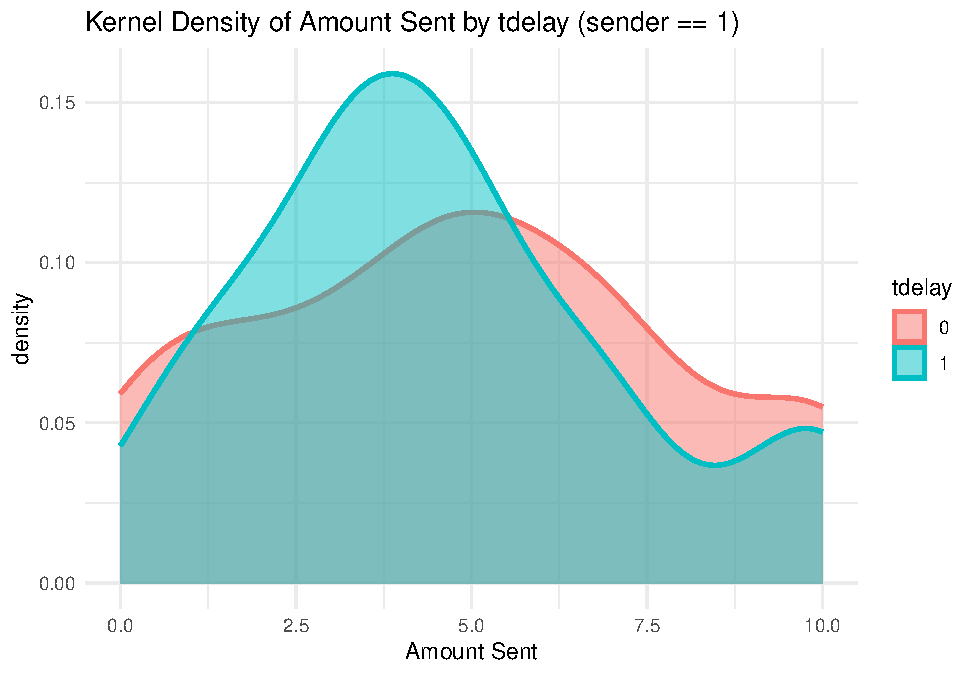
\includegraphics[keepaspectratio]{TrustOverRiskSimualtions_files/figure-latex/data_nature-1.pdf}}

\begin{Shaded}
\begin{Highlighting}[]
\CommentTok{\# Compute and print table with means of amountsent by tdelay group}
\NormalTok{means\_table }\OtherTok{\textless{}{-}}\NormalTok{ subset }\SpecialCharTok{\%\textgreater{}\%}
  \FunctionTok{group\_by}\NormalTok{(tdelay) }\SpecialCharTok{\%\textgreater{}\%}
  \FunctionTok{summarise}\NormalTok{(}
    \AttributeTok{n =} \FunctionTok{n}\NormalTok{(),}
    \AttributeTok{mean\_amountsent =} \FunctionTok{mean}\NormalTok{(amountsent, }\AttributeTok{na.rm =} \ConstantTok{TRUE}\NormalTok{)}
\NormalTok{  )}

\FunctionTok{print}\NormalTok{(means\_table)}
\end{Highlighting}
\end{Shaded}

\begin{verbatim}
## # A tibble: 2 x 3
##   tdelay     n mean_amountsent
##    <dbl> <int>           <dbl>
## 1      0    75            4.92
## 2      1    75            4.54
\end{verbatim}

\section{1.6 Power Analysis assuming continuous
disrtritbution}\label{power-analysis-assuming-continuous-disrtritbution}

We will now sample from a continuous distribution, and assume that the
treatment group is more likely to send higher amounts, and the control
group is more likely to send lower amounts. We assume that the design
effect is of 0.5/

\begin{Shaded}
\begin{Highlighting}[]
\CommentTok{\# SIMULATION 5}
\CommentTok{\# Define a sequence of n values}
\NormalTok{n\_values }\OtherTok{\textless{}{-}} \FunctionTok{seq}\NormalTok{(}\DecValTok{10}\NormalTok{, }\DecValTok{120}\NormalTok{, }\AttributeTok{by =} \DecValTok{5}\NormalTok{)}
\NormalTok{mean\_control }\OtherTok{\textless{}{-}} \DecValTok{5}
\NormalTok{mean\_treatment }\OtherTok{\textless{}{-}} \FloatTok{7.5}

\CommentTok{\# File paths for cached results}
\NormalTok{power\_results\_file }\OtherTok{\textless{}{-}} \StringTok{"power\_results\_sim5.rds"}

\ControlFlowTok{if}\NormalTok{ (}\FunctionTok{file.exists}\NormalTok{(power\_results\_file)) \{}
\NormalTok{  power\_results }\OtherTok{\textless{}{-}} \FunctionTok{readRDS}\NormalTok{(power\_results\_file)}
\NormalTok{\} }\ControlFlowTok{else}\NormalTok{ \{}
  \CommentTok{\# Prepare data frame to store results}
\NormalTok{  power\_results }\OtherTok{\textless{}{-}} \FunctionTok{data.frame}\NormalTok{(}
    \AttributeTok{n =} \FunctionTok{integer}\NormalTok{(),}
    \AttributeTok{t\_test\_power =} \FunctionTok{numeric}\NormalTok{(),}
    \AttributeTok{wilcox\_power =} \FunctionTok{numeric}\NormalTok{()}
\NormalTok{  )}

\NormalTok{  pb }\OtherTok{\textless{}{-}}\NormalTok{ progress\_bar}\SpecialCharTok{$}\FunctionTok{new}\NormalTok{(}
    \AttributeTok{format =} \StringTok{"  Simulating [:bar] :percent eta: :eta"}\NormalTok{,}
    \AttributeTok{total =} \FunctionTok{length}\NormalTok{(n\_values), }\AttributeTok{clear =} \ConstantTok{FALSE}\NormalTok{, }\AttributeTok{width =} \DecValTok{60}
\NormalTok{  )}
  \ControlFlowTok{for}\NormalTok{ (n }\ControlFlowTok{in}\NormalTok{ n\_values) \{}
    \CommentTok{\# t{-}test power}
\NormalTok{    t\_pvalues }\OtherTok{\textless{}{-}} \FunctionTok{numeric}\NormalTok{(reps)}
\NormalTok{    w\_pvalues }\OtherTok{\textless{}{-}} \FunctionTok{numeric}\NormalTok{(reps)}
    \ControlFlowTok{for}\NormalTok{ (i }\ControlFlowTok{in} \DecValTok{1}\SpecialCharTok{:}\NormalTok{reps) \{}
\NormalTok{      control }\OtherTok{\textless{}{-}} \FunctionTok{sample}\NormalTok{(}
        \FunctionTok{rnorm}\NormalTok{(n, }\AttributeTok{mean =}\NormalTok{ mean\_control, }\AttributeTok{sd =} \DecValTok{3}\NormalTok{), }
        \AttributeTok{size =}\NormalTok{ n, }
        \AttributeTok{replace =} \ConstantTok{TRUE}
\NormalTok{      )}
\NormalTok{      treatment }\OtherTok{\textless{}{-}} \FunctionTok{sample}\NormalTok{(}
        \FunctionTok{rnorm}\NormalTok{(n, }\AttributeTok{mean =}\NormalTok{ mean\_treatment, }\AttributeTok{sd =} \DecValTok{3}\NormalTok{), }
        \AttributeTok{size =}\NormalTok{ n, }
        \AttributeTok{replace =} \ConstantTok{TRUE}
\NormalTok{      )}
\NormalTok{      t\_pvalues[i] }\OtherTok{\textless{}{-}} \FunctionTok{t.test}\NormalTok{(control, treatment)}\SpecialCharTok{$}\NormalTok{p.value}
\NormalTok{      w\_pvalues[i] }\OtherTok{\textless{}{-}} \FunctionTok{wilcox.exact}\NormalTok{(control, treatment)}\SpecialCharTok{$}\NormalTok{p.value}
\NormalTok{    \}}
\NormalTok{    t\_test\_power }\OtherTok{\textless{}{-}} \FunctionTok{mean}\NormalTok{(t\_pvalues }\SpecialCharTok{\textless{}} \FloatTok{0.05}\NormalTok{)}
\NormalTok{    wilcox\_power }\OtherTok{\textless{}{-}} \FunctionTok{mean}\NormalTok{(w\_pvalues }\SpecialCharTok{\textless{}} \FloatTok{0.05}\NormalTok{)}
    \CommentTok{\# Store results}
\NormalTok{    power\_results }\OtherTok{\textless{}{-}} \FunctionTok{rbind}\NormalTok{(}
\NormalTok{      power\_results,}
      \FunctionTok{data.frame}\NormalTok{(}\AttributeTok{n =}\NormalTok{ n, }\AttributeTok{t\_test\_power =}\NormalTok{ t\_test\_power, }\AttributeTok{wilcox\_power =}\NormalTok{ wilcox\_power)}
\NormalTok{    )}
\NormalTok{    pb}\SpecialCharTok{$}\FunctionTok{tick}\NormalTok{()}
\NormalTok{  \}}
  \FunctionTok{saveRDS}\NormalTok{(power\_results, power\_results\_file)}
\NormalTok{\}}

\CommentTok{\# Reshape for plotting}
\FunctionTok{library}\NormalTok{(tidyr)}
\NormalTok{power\_long }\OtherTok{\textless{}{-}} \FunctionTok{pivot\_longer}\NormalTok{(power\_results, }\AttributeTok{cols =} \FunctionTok{c}\NormalTok{(}\StringTok{"t\_test\_power"}\NormalTok{, }\StringTok{"wilcox\_power"}\NormalTok{),}
                           \AttributeTok{names\_to =} \StringTok{"test"}\NormalTok{, }\AttributeTok{values\_to =} \StringTok{"power"}\NormalTok{)}

\CommentTok{\# Plot}
\FunctionTok{library}\NormalTok{(ggplot2)}
\FunctionTok{ggplot}\NormalTok{(power\_long, }\FunctionTok{aes}\NormalTok{(}\AttributeTok{x =}\NormalTok{ n, }\AttributeTok{y =}\NormalTok{ power, }\AttributeTok{color =}\NormalTok{ test)) }\SpecialCharTok{+}
  \FunctionTok{geom\_line}\NormalTok{(}\AttributeTok{size =} \FloatTok{1.2}\NormalTok{) }\SpecialCharTok{+}
  \FunctionTok{geom\_point}\NormalTok{(}\AttributeTok{size =} \DecValTok{2}\NormalTok{) }\SpecialCharTok{+}
  \FunctionTok{labs}\NormalTok{(}
    \AttributeTok{title =} \StringTok{"Power Curve for t{-}test and Wilcoxon Test"}\NormalTok{,}
    \AttributeTok{x =} \StringTok{"Sample Size (n)"}\NormalTok{,}
    \AttributeTok{y =} \StringTok{"Power (P{-}value \textgreater{} 0.05)"}\NormalTok{,}
    \AttributeTok{color =} \StringTok{"Test"}
\NormalTok{  ) }\SpecialCharTok{+}
  \FunctionTok{scale\_color\_manual}\NormalTok{(}\AttributeTok{values =} \FunctionTok{c}\NormalTok{(}\StringTok{"t\_test\_power"} \OtherTok{=} \StringTok{"\#1b9e77"}\NormalTok{, }\StringTok{"wilcox\_power"} \OtherTok{=} \StringTok{"\#d95f02"}\NormalTok{),}
                     \AttributeTok{labels =} \FunctionTok{c}\NormalTok{(}\StringTok{"t\_test\_power"} \OtherTok{=} \StringTok{"t{-}test"}\NormalTok{, }\StringTok{"wilcox\_power"} \OtherTok{=} \StringTok{"Wilcoxon"}\NormalTok{)) }\SpecialCharTok{+}
  \FunctionTok{theme\_minimal}\NormalTok{(}\AttributeTok{base\_size =} \DecValTok{14}\NormalTok{, }\AttributeTok{base\_family =} \StringTok{"Times"}\NormalTok{) }\SpecialCharTok{+}
  \FunctionTok{theme}\NormalTok{(}\AttributeTok{panel.grid =} \FunctionTok{element\_blank}\NormalTok{())}
\end{Highlighting}
\end{Shaded}

\pandocbounded{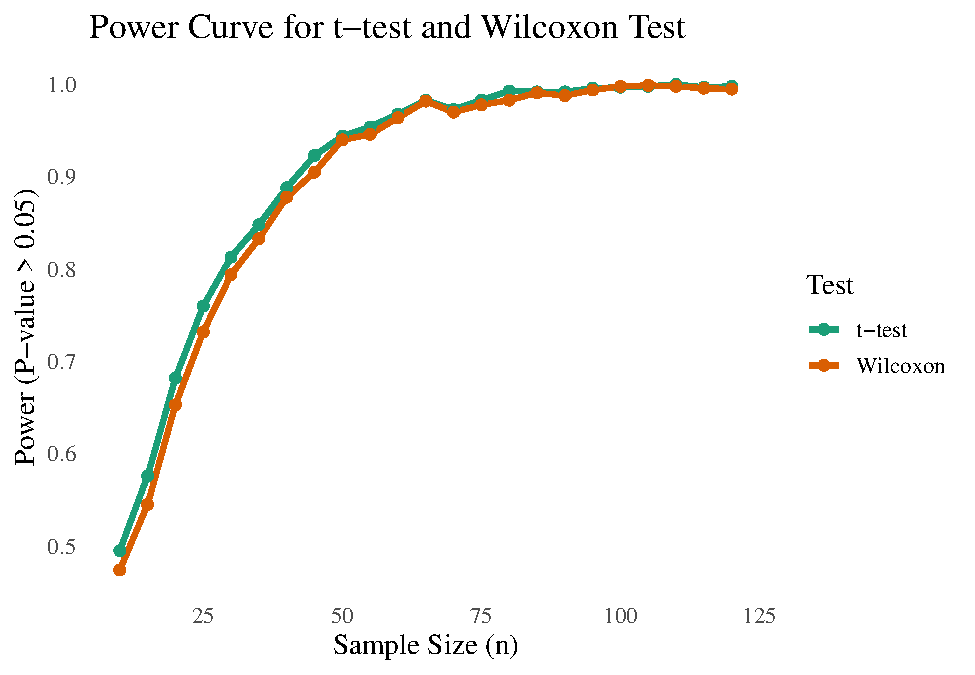
\includegraphics[keepaspectratio]{TrustOverRiskSimualtions_files/figure-latex/5-1.pdf}}

\begin{Shaded}
\begin{Highlighting}[]
\CommentTok{\# Print the power results as a LaTeX table}
\NormalTok{knitr}\SpecialCharTok{::}\FunctionTok{kable}\NormalTok{(}
\NormalTok{  power\_results,}
  \AttributeTok{format =} \StringTok{"latex"}\NormalTok{,}
  \AttributeTok{booktabs =} \ConstantTok{TRUE}\NormalTok{,}
  \AttributeTok{caption =} \StringTok{"Power Results for t{-}test and Wilcoxon Test Across Sample Sizes"}
\NormalTok{)}
\end{Highlighting}
\end{Shaded}

\begin{table}

\caption{\label{tab:5}Power Results for t-test and Wilcoxon Test Across Sample Sizes}
\centering
\begin{tabular}[t]{rrr}
\toprule
n & t\_test\_power & wilcox\_power\\
\midrule
10 & 0.495 & 0.474\\
15 & 0.576 & 0.545\\
20 & 0.682 & 0.653\\
25 & 0.760 & 0.732\\
30 & 0.813 & 0.794\\
\addlinespace
35 & 0.848 & 0.833\\
40 & 0.888 & 0.878\\
45 & 0.923 & 0.905\\
50 & 0.944 & 0.940\\
55 & 0.954 & 0.946\\
\addlinespace
60 & 0.968 & 0.964\\
65 & 0.983 & 0.982\\
70 & 0.973 & 0.970\\
75 & 0.983 & 0.978\\
80 & 0.993 & 0.983\\
\addlinespace
85 & 0.992 & 0.991\\
90 & 0.992 & 0.988\\
95 & 0.996 & 0.994\\
100 & 0.997 & 0.998\\
105 & 0.998 & 0.999\\
\addlinespace
110 & 1.000 & 0.998\\
115 & 0.997 & 0.996\\
120 & 0.998 & 0.995\\
\bottomrule
\end{tabular}
\end{table}

\begin{Shaded}
\begin{Highlighting}[]
\CommentTok{\# SIMULATION 6}
\CommentTok{\# Simulate interaction: probability of having an LLM account is higher in the treatment group}

\FunctionTok{set.seed}\NormalTok{(}\DecValTok{123}\NormalTok{) }\CommentTok{\# for reproducibility}
\NormalTok{n }\OtherTok{=} \DecValTok{100}
\NormalTok{mean\_control }\OtherTok{\textless{}{-}} \DecValTok{5}
\NormalTok{mean\_treatment }\OtherTok{\textless{}{-}} \FloatTok{7.5}

\CommentTok{\# File paths for cached results}
\NormalTok{reg\_pvalues\_int\_file }\OtherTok{\textless{}{-}} \StringTok{"reg\_pvalues\_int\_sim6.rds"}
\NormalTok{wilcox\_pvalues\_by\_llm\_file }\OtherTok{\textless{}{-}} \StringTok{"wilcox\_pvalues\_by\_llm\_sim6.rds"}

\ControlFlowTok{if}\NormalTok{ (}\FunctionTok{file.exists}\NormalTok{(reg\_pvalues\_int\_file) }\SpecialCharTok{\&\&} \FunctionTok{file.exists}\NormalTok{(wilcox\_pvalues\_by\_llm\_file)) \{}
\NormalTok{  reg\_pvalues\_int }\OtherTok{\textless{}{-}} \FunctionTok{readRDS}\NormalTok{(reg\_pvalues\_int\_file)}
\NormalTok{  wilcox\_pvalues\_by\_llm }\OtherTok{\textless{}{-}} \FunctionTok{readRDS}\NormalTok{(wilcox\_pvalues\_by\_llm\_file)}
\NormalTok{\} }\ControlFlowTok{else}\NormalTok{ \{}
\NormalTok{  reg\_pvalues\_int }\OtherTok{\textless{}{-}} \FunctionTok{data.frame}\NormalTok{(}
    \AttributeTok{group\_treatment =} \FunctionTok{numeric}\NormalTok{(reps),}
    \AttributeTok{llm\_account =} \FunctionTok{numeric}\NormalTok{(reps),}
    \AttributeTok{interaction =} \FunctionTok{numeric}\NormalTok{(reps)}
\NormalTok{  )}

\NormalTok{  wilcox\_pvalues\_by\_llm }\OtherTok{\textless{}{-}} \FunctionTok{data.frame}\NormalTok{(}
    \AttributeTok{rep =} \DecValTok{1}\SpecialCharTok{:}\NormalTok{reps,}
    \AttributeTok{llm0 =} \ConstantTok{NA\_real\_}\NormalTok{,}
    \AttributeTok{llm1 =} \ConstantTok{NA\_real\_}
\NormalTok{  )}

\NormalTok{  pb }\OtherTok{\textless{}{-}}\NormalTok{ progress\_bar}\SpecialCharTok{$}\FunctionTok{new}\NormalTok{(}
    \AttributeTok{format =} \StringTok{"  Simulating [:bar] :percent eta: :eta"}\NormalTok{,}
    \AttributeTok{total =}\NormalTok{ reps, }\AttributeTok{clear =} \ConstantTok{FALSE}\NormalTok{, }\AttributeTok{width =} \DecValTok{60}
\NormalTok{  )}
  \ControlFlowTok{for}\NormalTok{ (i }\ControlFlowTok{in} \DecValTok{1}\SpecialCharTok{:}\NormalTok{reps) \{}
    \CommentTok{\# Sample control group (baseline)}
\NormalTok{    control\_sent }\OtherTok{\textless{}{-}} \FunctionTok{sample}\NormalTok{(}
      \FunctionTok{rnorm}\NormalTok{(n, }\AttributeTok{mean =}\NormalTok{ mean\_control, }\AttributeTok{sd =} \DecValTok{3}\NormalTok{), }
      \AttributeTok{size =}\NormalTok{ n, }
      \AttributeTok{replace =} \ConstantTok{TRUE}
\NormalTok{    )}

    \CommentTok{\# Probability of LLM account increases with sent amount (e.g., logistic or linear scaling)}
\NormalTok{    control\_llm\_prob }\OtherTok{\textless{}{-}}\NormalTok{ scales}\SpecialCharTok{::}\FunctionTok{rescale}\NormalTok{(control\_sent, }\AttributeTok{to =} \FunctionTok{c}\NormalTok{(}\FloatTok{0.2}\NormalTok{, }\FloatTok{0.7}\NormalTok{)) }\CommentTok{\# adjust range as needed}
\NormalTok{    control\_llm\_account }\OtherTok{\textless{}{-}} \FunctionTok{rbinom}\NormalTok{(n, }\DecValTok{1}\NormalTok{, }\AttributeTok{prob =}\NormalTok{ control\_llm\_prob)}

    \CommentTok{\# Sample treatment group (LLM treatment)}
\NormalTok{    treatment\_sent }\OtherTok{\textless{}{-}} \FunctionTok{sample}\NormalTok{(}
      \FunctionTok{rnorm}\NormalTok{(n, }\AttributeTok{mean =}\NormalTok{ mean\_treatment, }\AttributeTok{sd =} \DecValTok{3}\NormalTok{), }
      \AttributeTok{size =}\NormalTok{ n, }
      \AttributeTok{replace =} \ConstantTok{TRUE}
\NormalTok{    )}

\NormalTok{    treatment\_llm\_prob }\OtherTok{\textless{}{-}}\NormalTok{ scales}\SpecialCharTok{::}\FunctionTok{rescale}\NormalTok{(treatment\_sent, }\AttributeTok{to =} \FunctionTok{c}\NormalTok{(}\FloatTok{0.4}\NormalTok{, }\FloatTok{0.95}\NormalTok{)) }\CommentTok{\# higher base probability}
\NormalTok{    treatment\_llm\_account }\OtherTok{\textless{}{-}} \FunctionTok{rbinom}\NormalTok{(n, }\DecValTok{1}\NormalTok{, }\AttributeTok{prob =}\NormalTok{ treatment\_llm\_prob)}

    \CommentTok{\# Combine into a single data frame}
\NormalTok{    sim\_data }\OtherTok{\textless{}{-}} \FunctionTok{data.frame}\NormalTok{(}
      \AttributeTok{group =} \FunctionTok{rep}\NormalTok{(}\FunctionTok{c}\NormalTok{(}\StringTok{"control"}\NormalTok{, }\StringTok{"treatment"}\NormalTok{), }\AttributeTok{each =}\NormalTok{ n),}
      \AttributeTok{sent =} \FunctionTok{c}\NormalTok{(control\_sent, treatment\_sent),}
      \AttributeTok{llm\_account =} \FunctionTok{c}\NormalTok{(control\_llm\_account, treatment\_llm\_account)}
\NormalTok{    )}

    \CommentTok{\# Fit linear regression: sent \textasciitilde{} group + llm\_account + group:llm\_account}
\NormalTok{    sim\_data}\SpecialCharTok{$}\NormalTok{group }\OtherTok{\textless{}{-}} \FunctionTok{factor}\NormalTok{(sim\_data}\SpecialCharTok{$}\NormalTok{group, }\AttributeTok{levels =} \FunctionTok{c}\NormalTok{(}\StringTok{"control"}\NormalTok{, }\StringTok{"treatment"}\NormalTok{))}
\NormalTok{    fit }\OtherTok{\textless{}{-}} \FunctionTok{lm}\NormalTok{(sent }\SpecialCharTok{\textasciitilde{}}\NormalTok{ group }\SpecialCharTok{+}\NormalTok{ llm\_account }\SpecialCharTok{+}\NormalTok{ group}\SpecialCharTok{:}\NormalTok{llm\_account, }\AttributeTok{data =}\NormalTok{ sim\_data)}
\NormalTok{    reg\_summary }\OtherTok{\textless{}{-}} \FunctionTok{summary}\NormalTok{(fit)}\SpecialCharTok{$}\NormalTok{coefficients}

    \CommentTok{\# Extract p{-}values for group\_treatment, llm\_account, and interaction}
\NormalTok{    reg\_pvalues\_int}\SpecialCharTok{$}\NormalTok{group\_treatment[i] }\OtherTok{\textless{}{-}} \ControlFlowTok{if}\NormalTok{ (}\StringTok{"grouptreatment"} \SpecialCharTok{\%in\%} \FunctionTok{rownames}\NormalTok{(reg\_summary)) reg\_summary[}\StringTok{"grouptreatment"}\NormalTok{, }\StringTok{"Pr(\textgreater{}|t|)"}\NormalTok{] }\ControlFlowTok{else} \ConstantTok{NA}
\NormalTok{    reg\_pvalues\_int}\SpecialCharTok{$}\NormalTok{llm\_account[i] }\OtherTok{\textless{}{-}} \ControlFlowTok{if}\NormalTok{ (}\StringTok{"llm\_account"} \SpecialCharTok{\%in\%} \FunctionTok{rownames}\NormalTok{(reg\_summary)) reg\_summary[}\StringTok{"llm\_account"}\NormalTok{, }\StringTok{"Pr(\textgreater{}|t|)"}\NormalTok{] }\ControlFlowTok{else} \ConstantTok{NA}
\NormalTok{    reg\_pvalues\_int}\SpecialCharTok{$}\NormalTok{interaction[i] }\OtherTok{\textless{}{-}} \ControlFlowTok{if}\NormalTok{ (}\StringTok{"grouptreatment:llm\_account"} \SpecialCharTok{\%in\%} \FunctionTok{rownames}\NormalTok{(reg\_summary)) reg\_summary[}\StringTok{"grouptreatment:llm\_account"}\NormalTok{, }\StringTok{"Pr(\textgreater{}|t|)"}\NormalTok{] }\ControlFlowTok{else} \ConstantTok{NA}

    \CommentTok{\# Wilcoxon test between control and treatment groups, separately for each llm\_account value}
    \ControlFlowTok{for}\NormalTok{ (llm\_val }\ControlFlowTok{in} \FunctionTok{c}\NormalTok{(}\DecValTok{0}\NormalTok{, }\DecValTok{1}\NormalTok{)) \{}
\NormalTok{      subset\_data }\OtherTok{\textless{}{-}}\NormalTok{ sim\_data[sim\_data}\SpecialCharTok{$}\NormalTok{llm\_account }\SpecialCharTok{==}\NormalTok{ llm\_val, ]}
      \ControlFlowTok{if}\NormalTok{ (}\FunctionTok{length}\NormalTok{(}\FunctionTok{unique}\NormalTok{(subset\_data}\SpecialCharTok{$}\NormalTok{group)) }\SpecialCharTok{==} \DecValTok{2}\NormalTok{) \{}
\NormalTok{        wilcox\_res }\OtherTok{\textless{}{-}} \FunctionTok{wilcox.exact}\NormalTok{(sent }\SpecialCharTok{\textasciitilde{}}\NormalTok{ group, }\AttributeTok{data =}\NormalTok{ subset\_data)}
\NormalTok{        wilcox\_pvalues\_by\_llm[i, }\FunctionTok{paste0}\NormalTok{(}\StringTok{"llm"}\NormalTok{, llm\_val)] }\OtherTok{\textless{}{-}}\NormalTok{ wilcox\_res}\SpecialCharTok{$}\NormalTok{p.value}
\NormalTok{      \}}
\NormalTok{    \}}
\NormalTok{    pb}\SpecialCharTok{$}\FunctionTok{tick}\NormalTok{()}
\NormalTok{  \}}

  \FunctionTok{saveRDS}\NormalTok{(reg\_pvalues\_int, reg\_pvalues\_int\_file)}
  \FunctionTok{saveRDS}\NormalTok{(wilcox\_pvalues\_by\_llm, wilcox\_pvalues\_by\_llm\_file)}
\NormalTok{\}}

\CommentTok{\# Power of the tests}
\NormalTok{power\_results\_int }\OtherTok{\textless{}{-}} \FunctionTok{data.frame}\NormalTok{(}
  \AttributeTok{Test =} \FunctionTok{c}\NormalTok{(}
    \StringTok{"t{-}test (group)"}\NormalTok{, }
    \StringTok{"t{-}test (interaction)"}\NormalTok{, }
    \StringTok{"Wilcoxon Exact (llm\_account=0)"}\NormalTok{, }
    \StringTok{"Wilcoxon Exact (llm\_account=1)"}
\NormalTok{  ),}
  \AttributeTok{Power =} \FunctionTok{c}\NormalTok{(}
    \FunctionTok{round}\NormalTok{(}\FunctionTok{mean}\NormalTok{(reg\_pvalues\_int}\SpecialCharTok{$}\NormalTok{group\_treatment }\SpecialCharTok{\textless{}} \FloatTok{0.05}\NormalTok{, }\AttributeTok{na.rm =} \ConstantTok{TRUE}\NormalTok{), }\DecValTok{3}\NormalTok{),}
    \FunctionTok{round}\NormalTok{(}\FunctionTok{mean}\NormalTok{(reg\_pvalues\_int}\SpecialCharTok{$}\NormalTok{interaction }\SpecialCharTok{\textless{}} \FloatTok{0.05}\NormalTok{, }\AttributeTok{na.rm =} \ConstantTok{TRUE}\NormalTok{), }\DecValTok{3}\NormalTok{),}
    \FunctionTok{round}\NormalTok{(}\FunctionTok{mean}\NormalTok{(wilcox\_pvalues\_by\_llm}\SpecialCharTok{$}\NormalTok{llm0 }\SpecialCharTok{\textless{}} \FloatTok{0.05}\NormalTok{, }\AttributeTok{na.rm =} \ConstantTok{TRUE}\NormalTok{), }\DecValTok{3}\NormalTok{),}
    \FunctionTok{round}\NormalTok{(}\FunctionTok{mean}\NormalTok{(wilcox\_pvalues\_by\_llm}\SpecialCharTok{$}\NormalTok{llm1 }\SpecialCharTok{\textless{}} \FloatTok{0.05}\NormalTok{, }\AttributeTok{na.rm =} \ConstantTok{TRUE}\NormalTok{), }\DecValTok{3}\NormalTok{)}
\NormalTok{  )}
\NormalTok{)}

\FunctionTok{print}\NormalTok{(power\_results\_int)}
\end{Highlighting}
\end{Shaded}

\begin{verbatim}
##                             Test Power
## 1                 t-test (group) 0.612
## 2           t-test (interaction) 0.059
## 3 Wilcoxon Exact (llm_account=0) 0.597
## 4 Wilcoxon Exact (llm_account=1) 0.826
\end{verbatim}

\section{Simulating Punishment
Decisions}\label{simulating-punishment-decisions}

\begin{Shaded}
\begin{Highlighting}[]
\CommentTok{\# SIMULATION 7: Punishment Decisions {-} Treatment vs Control}

\FunctionTok{set.seed}\NormalTok{(}\DecValTok{123}\NormalTok{) }\CommentTok{\# for reproducibility}
\NormalTok{n }\OtherTok{\textless{}{-}} \DecValTok{100}
\NormalTok{reps }\OtherTok{\textless{}{-}} \DecValTok{1000}
\NormalTok{mean\_treatment }\OtherTok{\textless{}{-}} \DecValTok{0}
\NormalTok{mean\_control }\OtherTok{\textless{}{-}} \FloatTok{1.5}
\NormalTok{sd\_punishment }\OtherTok{\textless{}{-}} \FloatTok{0.5}

\CommentTok{\# File paths for cached results}
\NormalTok{reg\_pvalues\_file }\OtherTok{\textless{}{-}} \StringTok{"reg\_pvalues\_sim7.rds"}
\NormalTok{wilcox\_pvalues\_file }\OtherTok{\textless{}{-}} \StringTok{"wilcox\_pvalues\_sim7.rds"}
\NormalTok{last\_sim\_data\_file }\OtherTok{\textless{}{-}} \StringTok{"last\_sim\_data\_sim7.rds"}

\ControlFlowTok{if}\NormalTok{ (}\FunctionTok{file.exists}\NormalTok{(reg\_pvalues\_file) }\SpecialCharTok{\&\&} \FunctionTok{file.exists}\NormalTok{(wilcox\_pvalues\_file) }\SpecialCharTok{\&\&} \FunctionTok{file.exists}\NormalTok{(last\_sim\_data\_file)) \{}
\NormalTok{  reg\_pvalues }\OtherTok{\textless{}{-}} \FunctionTok{readRDS}\NormalTok{(reg\_pvalues\_file)}
\NormalTok{  wilcox\_pvalues }\OtherTok{\textless{}{-}} \FunctionTok{readRDS}\NormalTok{(wilcox\_pvalues\_file)}
\NormalTok{  last\_sim\_data }\OtherTok{\textless{}{-}} \FunctionTok{readRDS}\NormalTok{(last\_sim\_data\_file)}
\NormalTok{\} }\ControlFlowTok{else}\NormalTok{ \{}
\NormalTok{  reg\_pvalues }\OtherTok{\textless{}{-}} \FunctionTok{numeric}\NormalTok{(reps)}
\NormalTok{  wilcox\_pvalues }\OtherTok{\textless{}{-}} \FunctionTok{numeric}\NormalTok{(reps)}
\NormalTok{  last\_sim\_data }\OtherTok{\textless{}{-}} \ConstantTok{NULL}

\NormalTok{  pb }\OtherTok{\textless{}{-}}\NormalTok{ progress\_bar}\SpecialCharTok{$}\FunctionTok{new}\NormalTok{(}
    \AttributeTok{format =} \StringTok{"  Simulating [:bar] :percent eta: :eta"}\NormalTok{,}
    \AttributeTok{total =}\NormalTok{ reps, }\AttributeTok{clear =} \ConstantTok{FALSE}\NormalTok{, }\AttributeTok{width =} \DecValTok{60}
\NormalTok{  )}

  \ControlFlowTok{for}\NormalTok{ (i }\ControlFlowTok{in} \DecValTok{1}\SpecialCharTok{:}\NormalTok{reps) \{}
\NormalTok{    punishment\_treatment }\OtherTok{\textless{}{-}} \FunctionTok{rnorm}\NormalTok{(n, }\AttributeTok{mean =}\NormalTok{ mean\_treatment, }\AttributeTok{sd =}\NormalTok{ sd\_punishment)}
\NormalTok{    punishment\_control }\OtherTok{\textless{}{-}} \FunctionTok{rnorm}\NormalTok{(n, }\AttributeTok{mean =}\NormalTok{ mean\_control, }\AttributeTok{sd =}\NormalTok{ sd\_punishment)}
\NormalTok{    group }\OtherTok{\textless{}{-}} \FunctionTok{factor}\NormalTok{(}\FunctionTok{rep}\NormalTok{(}\FunctionTok{c}\NormalTok{(}\StringTok{"treatment"}\NormalTok{, }\StringTok{"control"}\NormalTok{), }\AttributeTok{each =}\NormalTok{ n), }\AttributeTok{levels =} \FunctionTok{c}\NormalTok{(}\StringTok{"control"}\NormalTok{, }\StringTok{"treatment"}\NormalTok{))}
\NormalTok{    punishment }\OtherTok{\textless{}{-}} \FunctionTok{c}\NormalTok{(punishment\_treatment, punishment\_control)}
\NormalTok{    sim\_data }\OtherTok{\textless{}{-}} \FunctionTok{data.frame}\NormalTok{(}
      \AttributeTok{group =}\NormalTok{ group,}
      \AttributeTok{punishment =}\NormalTok{ punishment}
\NormalTok{    )}

    \CommentTok{\# Linear regression: punishment \textasciitilde{} group}
\NormalTok{    fit }\OtherTok{\textless{}{-}} \FunctionTok{lm}\NormalTok{(punishment }\SpecialCharTok{\textasciitilde{}}\NormalTok{ group, }\AttributeTok{data =}\NormalTok{ sim\_data)}
\NormalTok{    reg\_summary }\OtherTok{\textless{}{-}} \FunctionTok{summary}\NormalTok{(fit)}\SpecialCharTok{$}\NormalTok{coefficients}
\NormalTok{    reg\_pvalues[i] }\OtherTok{\textless{}{-}} \ControlFlowTok{if}\NormalTok{ (}\StringTok{"grouptreatment"} \SpecialCharTok{\%in\%} \FunctionTok{rownames}\NormalTok{(reg\_summary)) reg\_summary[}\StringTok{"grouptreatment"}\NormalTok{, }\StringTok{"Pr(\textgreater{}|t|)"}\NormalTok{] }\ControlFlowTok{else} \ConstantTok{NA}

    \CommentTok{\# Wilcoxon exact test}
\NormalTok{    wilcox\_res }\OtherTok{\textless{}{-}} \FunctionTok{wilcox.exact}\NormalTok{(punishment }\SpecialCharTok{\textasciitilde{}}\NormalTok{ group, }\AttributeTok{data =}\NormalTok{ sim\_data)}
\NormalTok{    wilcox\_pvalues[i] }\OtherTok{\textless{}{-}}\NormalTok{ wilcox\_res}\SpecialCharTok{$}\NormalTok{p.value}

    \CommentTok{\# Store the last simulation data for plotting}
    \ControlFlowTok{if}\NormalTok{ (i }\SpecialCharTok{==}\NormalTok{ reps) last\_sim\_data }\OtherTok{\textless{}{-}}\NormalTok{ sim\_data}

\NormalTok{    pb}\SpecialCharTok{$}\FunctionTok{tick}\NormalTok{()}
\NormalTok{  \}}

  \FunctionTok{saveRDS}\NormalTok{(reg\_pvalues, reg\_pvalues\_file)}
  \FunctionTok{saveRDS}\NormalTok{(wilcox\_pvalues, wilcox\_pvalues\_file)}
  \FunctionTok{saveRDS}\NormalTok{(last\_sim\_data, last\_sim\_data\_file)}
\NormalTok{\}}

\CommentTok{\# Print summary of p{-}values}
\FunctionTok{cat}\NormalTok{(}\StringTok{"Proportion of significant results (p \textless{} 0.05):}\SpecialCharTok{\textbackslash{}n}\StringTok{"}\NormalTok{)}
\end{Highlighting}
\end{Shaded}

\begin{verbatim}
## Proportion of significant results (p < 0.05):
\end{verbatim}

\begin{Shaded}
\begin{Highlighting}[]
\FunctionTok{cat}\NormalTok{(}\StringTok{"Linear regression:"}\NormalTok{, }\FunctionTok{mean}\NormalTok{(reg\_pvalues }\SpecialCharTok{\textless{}} \FloatTok{0.05}\NormalTok{, }\AttributeTok{na.rm =} \ConstantTok{TRUE}\NormalTok{), }\StringTok{"}\SpecialCharTok{\textbackslash{}n}\StringTok{"}\NormalTok{)}
\end{Highlighting}
\end{Shaded}

\begin{verbatim}
## Linear regression: 1
\end{verbatim}

\begin{Shaded}
\begin{Highlighting}[]
\FunctionTok{cat}\NormalTok{(}\StringTok{"Wilcoxon exact:"}\NormalTok{, }\FunctionTok{mean}\NormalTok{(wilcox\_pvalues }\SpecialCharTok{\textless{}} \FloatTok{0.05}\NormalTok{, }\AttributeTok{na.rm =} \ConstantTok{TRUE}\NormalTok{), }\StringTok{"}\SpecialCharTok{\textbackslash{}n}\StringTok{"}\NormalTok{)}
\end{Highlighting}
\end{Shaded}

\begin{verbatim}
## Wilcoxon exact: 1
\end{verbatim}

\begin{Shaded}
\begin{Highlighting}[]
\CommentTok{\# Plot kernel density of punishment for last simulation}
\FunctionTok{library}\NormalTok{(ggplot2)}
\FunctionTok{ggplot}\NormalTok{(last\_sim\_data, }\FunctionTok{aes}\NormalTok{(}\AttributeTok{x =}\NormalTok{ punishment, }\AttributeTok{fill =}\NormalTok{ group, }\AttributeTok{color =}\NormalTok{ group)) }\SpecialCharTok{+}
  \FunctionTok{geom\_density}\NormalTok{(}\AttributeTok{alpha =} \FloatTok{0.4}\NormalTok{, }\AttributeTok{size =} \DecValTok{1}\NormalTok{) }\SpecialCharTok{+}
  \FunctionTok{scale\_fill\_manual}\NormalTok{(}\AttributeTok{values =} \FunctionTok{c}\NormalTok{(}\StringTok{"control"} \OtherTok{=} \StringTok{"\#1b9e77"}\NormalTok{, }\StringTok{"treatment"} \OtherTok{=} \StringTok{"\#d95f02"}\NormalTok{)) }\SpecialCharTok{+}
  \FunctionTok{scale\_color\_manual}\NormalTok{(}\AttributeTok{values =} \FunctionTok{c}\NormalTok{(}\StringTok{"control"} \OtherTok{=} \StringTok{"\#1b9e77"}\NormalTok{, }\StringTok{"treatment"} \OtherTok{=} \StringTok{"\#d95f02"}\NormalTok{)) }\SpecialCharTok{+}
  \FunctionTok{labs}\NormalTok{(}
    \AttributeTok{title =} \StringTok{"Kernel Density of Punishment: Control vs. Treatment (Last Simulation)"}\NormalTok{,}
    \AttributeTok{x =} \StringTok{"Punishment"}\NormalTok{,}
    \AttributeTok{y =} \StringTok{"Density"}\NormalTok{,}
    \AttributeTok{fill =} \StringTok{"Group"}\NormalTok{,}
    \AttributeTok{color =} \StringTok{"Group"}
\NormalTok{  ) }\SpecialCharTok{+}
  \FunctionTok{theme\_minimal}\NormalTok{(}\AttributeTok{base\_size =} \DecValTok{14}\NormalTok{) }\SpecialCharTok{+}
  \FunctionTok{theme}\NormalTok{(}\AttributeTok{panel.grid =} \FunctionTok{element\_blank}\NormalTok{())}
\end{Highlighting}
\end{Shaded}

\pandocbounded{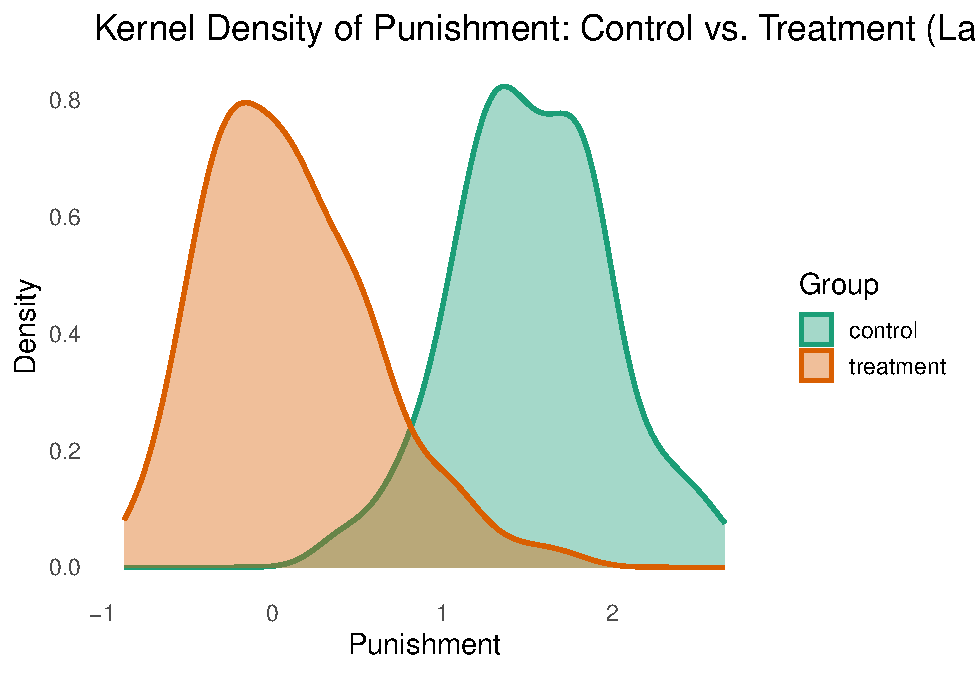
\includegraphics[keepaspectratio]{TrustOverRiskSimualtions_files/figure-latex/7-1.pdf}}

\end{document}
